\documentclass[11pt,oneside]{article}
\pdfminorversion=7
\usepackage{QuizStyle}
\usepackage{tikz}
\hypersetup{
  pdftitle={20261030 Midterm for MATH312 Analysis II},
  pdfauthor={Jungwoo Kim},
  pdfsubject={Rudin Chapters 7 and 8 exercises for MATH312 Analysis II},
  pdfcreator={LaTeX}
}
\begin{document}
\quiztitle{20261030 Midterm}

\begin{exercise}{7.1}
Prove that every uniformly convergent sequence of bounded functions is uniformly bounded.
\end{exercise}
\begin{solution}
Let $f_n\unifto f$ on $E$, with each $f_n$ bounded. Choose $N$ so that
$|f_n(x)-f_N(x)|<1$ for all $x\in E$ whenever $n\ge N$; this is possible by the uniform Cauchy criterion (Theorem 7.8). Since $f_N$ is bounded, say $|f_N(x)|\le M_N$, we have
\[
 |f_n(x)|\le |f_n(x)-f_N(x)|+|f_N(x)|\le 1+M_N
 \qquad (n\ge N, \ x\in E).
\]
The finitely many functions $f_1, \ldots, f_{N-1}$ also have finite bounds. Taking the maximum of all these bounds and $1+M_N$ produces a constant $M$ such that $|f_n(x)|\le M$ for every $n$ and every $x\in E$.
\end{solution}

\begin{exercise}{7.2}
If $(f_n)$ and $(g_n)$ converge uniformly on a set $E$, prove that $(f_n+g_n)$ converges uniformly on $E$. If, in addition, $(f_n)$ and $(g_n)$ are sequences of bounded functions, prove that $(f_ng_n)$ converges uniformly on $E$.
\end{exercise}
\begin{solution}
Write $f_n\unifto f$ and $g_n\unifto g$. For every $x\in E$,
\[
 |(f_n+g_n)(x)-(f+g)(x)|\le |f_n(x)-f(x)|+|g_n(x)-g(x)|.
\]
Taking suprema shows that the right side tends to $0$, so $f_n+g_n\unifto f+g$.

For products, Exercise 7.1 supplies constants $M_f, M_g$ with $|f_n|\le M_f$ and $|g_n|\le M_g$ on $E$ for all $n$. The pointwise limits satisfy $|f|\le M_f$ and $|g|\le M_g$. Thus
\[
 \begin{aligned}
 |f_n(x)g_n(x)-f(x)g(x)|
 &\le |f_n(x)|\,|g_n(x)-g(x)|+|g(x)|\,|f_n(x)-f(x)|\\
 &\le M_f|g_n(x)-g(x)|+M_g|f_n(x)-f(x)|.
 \end{aligned}
\]
Both terms tend to zero uniformly in $x$, proving $f_ng_n\unifto fg$.
\end{solution}

\begin{exercise}{7.3}
Construct sequences $(f_n)$, $(g_n)$ which converge uniformly on some set $E$, but such that $(f_ng_n)$ does not converge uniformly on $E$ (of course, $(f_ng_n)$ must converge on $E$).
\end{exercise}
\begin{solution}
Take $E=\R$, $f_n(x)=1/n$, and $g_n(x)=x$ for every $n$. Since $\sup_{x\in\R}|f_n(x)|=1/n\to0$, we have $f_n\unifto0$; the constant sequence $g_n=g$ converges uniformly to $g(x)=x$. However, $f_n(x)g_n(x)=x/n$ converges pointwise to $0$, while
\[
 \sup_{x\in\R}|x/n|=\infty\qquad(n\ge1).
\]
Consequently the products do not converge uniformly.
\end{solution}

\begin{exercise}{7.4}
Consider
\[
 f(x)=\sum_{n=1}^{\infty}\frac{1}{1+n^2x}.
\]
For what values of $x$ does the series converge absolutely? On what intervals does it converge uniformly? On what intervals does it fail to converge uniformly? Is $f$ continuous wherever the series converges? Is $f$ bounded?
\end{exercise}
\begin{solution}
The expression is undefined at $x=-1/n^2$ for any $n\ge1$. For $x=0$ every summand equals $1$, so the series diverges. For any fixed $x\ne0$ avoiding these poles,
\[
 \lim_{n\to\infty}n^2\left|\frac1{1+n^2x}\right|=\frac1{|x|}.
\]
Comparison with $\sum n^{-2}$ proves absolute convergence exactly on
\[
 D=\R\setminus\bigl(\{0\}\cup\{-1/n^2:n\ge1\}\bigr).
\]

For $x\ge a>0$, we have $0<(1+n^2x)^{-1}\le(a n^2)^{-1}$; the Weierstrass M-test (Theorem 7.10) gives uniform convergence on every interval contained in $[a, \infty)$. Likewise, if $x\le-a<0$ and $n^2a\ge2$, then
\[
 \left|\frac1{1+n^2x}\right|\le\frac2{a n^2}.
\]
Thus the tails converge uniformly on every interval in $(-\infty, -a]$ on which the terms are defined; finitely many earlier terms do not affect uniform convergence. More generally, the series converges uniformly on any subset of $D$ bounded away from $0$.

It fails to converge uniformly on $(0, b)$ for every $b>0$: for each fixed $N$, choosing $x>0$ sufficiently small makes each of the $N$ terms with $n=N, \ldots, 2N-1$ greater than $1/2$, so these tails cannot be uniformly small. No interval containing $0$ lies in $D$.

Every term is continuous on $D$, and the series is locally uniformly convergent there; Theorem 7.12 therefore gives continuity of $f$ at every point of $D$. Finally $f$ is unbounded: $f(x)\to\infty$ as $x\to0^+$, since any fixed number of its positive terms tends to $1$. It is also unbounded in neighborhoods of its negative poles within $D$.
\end{solution}

\begin{exercise}{7.5}
Let
\[
 f_n(x)=\begin{cases}
 0, &x<\dfrac1{n+1}, \\[3pt]
 \sin^2\!\dfrac{\pi}{x}, &\dfrac1{n+1}\le x\le\dfrac1n, \\[5pt]
 0, &\dfrac1n<x.
 \end{cases}
\]
Show that $(f_n)$ converges to a continuous function, but not uniformly. Use the series $\sum f_n$ to show that absolute convergence, even for all $x$, does not imply uniform convergence.
\end{exercise}
\begin{solution}
The function $f_n$ vanishes outside $[1/(n+1), 1/n]$ and at both endpoints of that interval. Thus each $f_n$ is continuous. For any fixed $x$, at most one $f_n(x)$ can be nonzero, so $f_n(x)\to0$. The limit function $f\equiv0$ is continuous.

On each interval $[1/(n+1), 1/n]$, the variable $1/x$ runs through $[n, n+1]$. In particular, at $x_n=1/(n+1/2)$,
\[
 f_n(x_n)=\sin^2\bigl(\pi(n+\tfrac12)\bigr)=1.
\]
Hence $\sup_{x\in\R}|f_n(x)|=1$ for every $n$, and Theorem 7.9 shows that the convergence is not uniform.

Since the supports are disjoint except at points where both neighboring functions vanish, $\sum_n|f_n(x)|=\sum_nf_n(x)$ has at most one nonzero term for every $x$: the series converges absolutely everywhere. But its tail satisfies
\[
 \sup_{x\in\R}\left|\sum_{n=N}^{\infty}f_n(x)\right|\ge f_N(x_N)=1.
\]
The series therefore fails the uniform Cauchy criterion, despite absolute convergence at every point.
\end{solution}

\begin{exercise}{7.6}
Prove that the series
\[
 \sum_{n=1}^{\infty}\frac{(-1)^n}{n^2}(x^2+n)
\]
converges uniformly in every bounded interval, but does not converge absolutely for any value of $x$.
\end{exercise}
\begin{solution}
Split the series as
\[
 \sum_{n=1}^{\infty}\frac{(-1)^n(x^2+n)}{n^2}
 =x^2\sum_{n=1}^{\infty}\frac{(-1)^n}{n^2}
  +\sum_{n=1}^{\infty}\frac{(-1)^n}{n}.
\]
The second series converges as an alternating numerical series and its partial sums do not depend on $x$. For $|x|\le B$, the tails of the first series satisfy
\[
 \sup_{|x|\le B}\left|x^2\sum_{n=N}^{M}\frac{(-1)^n}{n^2}\right|
 \le B^2\sum_{n=N}^{\infty}\frac1{n^2}\longrightarrow0.
\]
Thus both parts converge uniformly on $[-B, B]$, and hence on any bounded interval. On the other hand, for every fixed $x$,
\[
 \left|\frac{(-1)^n(x^2+n)}{n^2}\right|
 =\frac1n+\frac{x^2}{n^2}\ge\frac1n.
\]
The absolute-value series dominates the divergent harmonic series and therefore diverges for every $x$.
\end{solution}

\begin{exercise}{7.7}
For $n=1, 2, 3, \ldots$ and real $x$, put
\[
 f_n(x)=\frac{x}{1+nx^2}.
\]
Show that $(f_n)$ converges uniformly to a function $f$, and that the equation
\[
 f'(x)=\lim_{n\to\infty}f_n'(x)
\]
is correct if $x\ne0$, but false if $x=0$.
\end{exercise}
\begin{solution}
For every fixed $x$, $f_n(x)\to0$, so $f\equiv0$. To prove uniform convergence on $\R$, maximize $t/(1+nt^2)$ for $t\ge0$. Its derivative is $(1-nt^2)/(1+nt^2)^2$, which changes sign at $t=1/\sqrt n$. Therefore
\[
 \sup_{x\in\R}|f_n(x)|=\frac1{2\sqrt n}\longrightarrow0.
\]
Differentiating gives
\[
 f_n'(x)=\frac{1-nx^2}{(1+nx^2)^2}.
\]
For each fixed $x\ne0$ this tends to $0=f'(x)$. At $x=0$, however, $f_n'(0)=1$ for every $n$, whereas $f'(0)=0$.
\end{solution}

\begin{exercise}{7.8}
If
\[
 I(x)=\begin{cases}0, &x\le0, \\1, &x>0, \end{cases}
\]
if $(x_n)$ is a sequence of distinct points of $(a, b)$, and if $\sum|c_n|$ converges, prove that the series
\[
 f(x)=\sum_{n=1}^{\infty}c_n I(x-x_n)\qquad(a\le x\le b)
\]
converges uniformly and that $f$ is continuous for every $x\ne x_n$.
\end{exercise}
\begin{solution}
Since $|I(x-x_n)|\le1$,
\[
 |c_n I(x-x_n)|\le |c_n|\qquad(x\in[a, b]).
\]
The numerical series $\sum|c_n|$ converges; hence the Weierstrass M-test (Theorem 7.10) proves uniform convergence.

For a fixed $x\notin\{x_n:n\ge1\}$, each function $t\mapsto c_n I(t-x_n)$ is continuous at $x$: its only possible discontinuity occurs at $x_n$. Thus every partial sum is continuous at $x$. Uniform convergence allows the limit to be passed through $t\to x$ (Theorem 7.11), proving that $f$ is continuous at $x$.
\end{solution}

\begin{exercise}{7.9}
Let $(f_n)$ be a sequence of continuous functions which converges uniformly to a function $f$ on a set $E$. Prove that
\[
 \lim_{n\to\infty}f_n(x_n)=f(x)
\]
for every sequence of points $x_n\in E$ such that $x_n\to x$ and $x\in E$. Is the converse of this true?
\end{exercise}
\begin{solution}
The uniform limit $f$ is continuous on $E$ by Theorem 7.12. Therefore
\[
 \begin{aligned}
 |f_n(x_n)-f(x)|
 &\le |f_n(x_n)-f(x_n)|+|f(x_n)-f(x)|\\
 &\le\sup_{t\in E}|f_n(t)-f(t)|+|f(x_n)-f(x)|\longrightarrow0.
 \end{aligned}
\]
The first term tends to zero uniformly, and the second by continuity at $x$.

The converse is false on general sets. Let $E=\R$ and take
\[
 f_n(x)=\max\{1-|x-n|, 0\}, \qquad f(x)=0.
\]
Each $f_n$ is continuous. For every fixed $x$, $f_n(x)=0$ for all sufficiently large $n$, so $f_n\to f$ pointwise. If $x_n\to x\in\R$, the sequence $(x_n)$ is bounded, whereas the support of $f_n$ is $[n-1, n+1]$. Thus $f_n(x_n)=0$ eventually, giving the required limit. Nevertheless $\sup_{x\in\R}|f_n(x)-f(x)|=1$ for every $n$, so the convergence is not uniform.
\end{solution}

\begin{exercise}{7.10}
Letting $\{x\}$ denote the fractional part of the real number $x$ (see Exercise 16, Chap.~4, for the definition), consider the function
\[
 f(x)=\sum_{n=1}^{\infty}\frac{\{nx\}}{n^2}\qquad(x\in\R).
\]
Find all discontinuities of $f$, and show that they form a countable dense set. Show that $f$ is nevertheless Riemann-integrable on every bounded interval.
\end{exercise}
\begin{solution}
For every $n$ and $x$, $0\le\{nx\}<1$, so
\[
 \left|\frac{\{nx\}}{n^2}\right|\le\frac1{n^2}.
\]
The Weierstrass M-test (Theorem 7.10) gives uniform convergence on $\R$.

If $x$ is irrational, none of the numbers $nx$ is an integer. Therefore every summand is continuous at $x$, and uniform convergence (Theorem 7.11) implies that $f$ is continuous there.

Now let $x=p/q$ in lowest terms, with $q\ge1$. For $n$ divisible by $q$, the left-hand limit of $\{nt\}$ at $x$ equals $1$, while its value at $x$ equals $0$. For other $n$, the summand is continuous at $x$. Because the series converges uniformly, we may take the left-hand limit term by term and obtain
\[
 \lim_{t\to x^-}f(t)-f(x)
 =\sum_{m=1}^{\infty}\frac1{(mq)^2}>0.
\]
Hence every rational number is a discontinuity. The discontinuity set is exactly $\Q$, which is countable and dense in $\R$.

Finally, on any compact interval, each summand $x\mapsto\{nx\}/n^2$ is bounded and has only finitely many discontinuities, so it is Riemann-integrable. Its partial sums are Riemann-integrable, and they converge uniformly to $f$. The integration theorem for uniform limits (Theorem 7.16 with $\alpha(x)=x$) therefore shows that $f$ is Riemann-integrable on every bounded interval.
\end{solution}

\begin{exercise}{7.11}
Suppose $(f_n)$, $(g_n)$ are defined on $E$, and
\begin{exercisesubparts}
\item $\sum f_n$ has uniformly bounded partial sums;
\item $g_n\to0$ uniformly on $E$;
\item $g_1(x)\ge g_2(x)\ge g_3(x)\ge\cdots$ for every $x\in E$.
\end{exercisesubparts}
Prove that $\sum f_ng_n$ converges uniformly on $E$.
\end{exercise}
\begin{solution}
Let $S_m(x)=\sum_{n=1}^{m}f_n(x)$ and choose $C$ such that $|S_m(x)|\le C$ for every $m$ and $x$. Since $g_n(x)$ decreases to $0$, each $g_n(x)\ge0$.

Fix $N\le M$ and define $A_k(x)=\sum_{n=N}^k f_n(x)=S_k(x)-S_{N-1}(x)$. Then $|A_k(x)|\le2C$. Summation by parts, as in the proof of Dirichlet's test (Theorem 3.42), gives
\[
 \sum_{n=N}^{M}f_n(x)g_n(x)
 =A_M(x)g_M(x)+\sum_{k=N}^{M-1}A_k(x)\bigl(g_k(x)-g_{k+1}(x)\bigr).
\]
Because the differences $g_k-g_{k+1}$ are nonnegative,
\[
 \begin{aligned}
 \left|\sum_{n=N}^{M}f_n(x)g_n(x)\right|
 &\le 2C\left(g_M(x)+\sum_{k=N}^{M-1}(g_k(x)-g_{k+1}(x))\right)\\
 &=2C g_N(x).
 \end{aligned}
\]
The uniform convergence $g_N\to0$ makes this bound uniformly small for large $N$, independently of $M$ and $x$. The uniform Cauchy criterion (Theorem 7.8) now yields uniform convergence of $\sum f_ng_n$.
\end{solution}

\begin{exercise}{7.12}
Suppose $g$ and $f_n$ ($n=1, 2, 3, \ldots$) are defined on $(0, \infty)$, are Riemann-integrable on $[t, T]$ whenever $0<t<T<\infty$, $|f_n|\le g$, $f_n\to f$ uniformly on every compact subset of $(0, \infty)$, and
\[
 \int_0^{\infty}g(x)\,\dd x<\infty.
\]
Prove that
\[
 \lim_{n\to\infty}\int_0^{\infty}f_n(x)\,\dd x
 =\int_0^{\infty}f(x)\,\dd x.
\]
\end{exercise}
\begin{solution}
Taking pointwise limits in $|f_n|\le g$ gives $|f|\le g$, so $f$ has the same integrable majorant as the $f_n$. On every interval $[\delta, R]\subset(0, \infty)$, the limit $f$ is Riemann-integrable and
\[
 \int_\delta^R f_n(x)\,\dd x\longrightarrow\int_\delta^R f(x)\,\dd x
\]
by Theorem 7.16, since convergence is uniform there.

Let $\varepsilon>0$. Because the improper integral of the nonnegative function $g$ is finite, choose $0<\delta<R$ so that
\[
 \int_0^\delta g(x)\,\dd x+\int_R^\infty g(x)\,\dd x<\frac\varepsilon3.
\]
The integrals of $f_n$ and $f$ over the two tails exist absolutely and are bounded by the corresponding integrals of $g$. For sufficiently large $n$, uniform convergence on $[\delta, R]$ gives
\[
 \left|\int_\delta^R(f_n-f)\,\dd x\right|<\frac\varepsilon3.
\]
Therefore
\[
 \begin{aligned}
 \left|\int_0^\infty f_n\,\dd x-\int_0^\infty f\,\dd x\right|
 &\le\int_0^\delta(|f_n|+|f|)\,\dd x
 +\left|\int_\delta^R(f_n-f)\,\dd x\right|\\
 &\qquad+\int_R^\infty(|f_n|+|f|)\,\dd x
 <\varepsilon.
 \end{aligned}
\]
\end{solution}

\begin{exercise}{7.13}
Assume that $(f_n)$ is a sequence of monotonically increasing functions on $\R$ with $0\le f_n(x)\le1$ for all $x$ and all $n$.
\begin{exercisesubparts}
\item Prove that there is a function $f$ and a sequence $(n_k)$ such that
\[
 f(x)=\lim_{k\to\infty}f_{n_k}(x)
\]
for every $x\in\R$.
\item If, moreover, $f$ is continuous, prove that $f_{n_k}\to f$ uniformly on compact sets.
\end{exercisesubparts}
\end{exercise}
\begin{solution}
\begin{exercisesubparts}
\item Enumerate the rationals as $(r_j)$. Since $0\le f_n(r_1)\le1$, there is a subsequence along which $f_n(r_1)$ converges. Repeat for $r_2, r_3, \ldots$, choosing nested subsequences. The diagonal subsequence, denoted $(g_k)$, converges at every rational $r$; write $h(r)=\lim_k g_k(r)$. Because each $g_k$ is increasing, $h$ is increasing on $\Q$.

Define the nondecreasing function
\[
 F(x)=\sup\{h(r):r\in\Q, \ r\le x\}.
\]
At each continuity point $x$ of $F$, choose rationals $r<x<s$ close enough that $h(s)-h(r)$ is as small as desired. For every $k$, monotonicity yields
\[
 g_k(r)\le g_k(x)\le g_k(s).
\]
Passing to the limit in the outer terms traps $g_k(x)$ between numbers arbitrarily close to $F(x)$, and hence $g_k(x)\to F(x)$.

A monotone real function has at most countably many discontinuities. Enumerate those of $F$ as $(d_j)$ and repeat the nested-subsequence and diagonal argument at the points $d_j$. This produces a further subsequence $(g_{k_j})$ converging at every discontinuity of $F$; it continues to converge to $F$ at every continuity point. Define $f(x)=\lim_jg_{k_j}(x)$ at all $x$. Then $f$ is defined everywhere and is the required pointwise limit. Its possible values at the discontinuities need not equal the initially chosen values of $F$, which is why the second diagonal selection is needed.

\item Suppose this pointwise limit $f$ is continuous, and let $[a, b]$ be any compact interval. Because $f$ is continuous and nondecreasing, it is uniformly continuous. Given $\varepsilon>0$, choose a partition
\[
 a=t_0<t_1<\cdots<t_m=b
\]
so fine that $f(t_i)-f(t_{i-1})<\varepsilon$. Pointwise convergence at the finitely many endpoints gives $N$ such that $|f_{n_k}(t_i)-f(t_i)|<\varepsilon$ for every $i$ whenever $k\ge N$. If $t_{i-1}\le x\le t_i$, the monotonicity of $f_{n_k}$ and $f$ then gives
\[
 f(x)-2\varepsilon\le f_{n_k}(x)\le f(x)+2\varepsilon.
\]
Thus $\sup_{x\in[a, b]}|f_{n_k}(x)-f(x)|\le2\varepsilon$ for $k\ge N$. This proves uniform convergence on every compact interval.
\end{exercisesubparts}
\end{solution}

\begin{exercise}{7.14}
Let $f$ be a continuous real function on $\R$ with the following properties: $0\le f(t)\le1$, $f(t+2)=f(t)$ for every $t$, and
\[
 f(t)=\begin{cases}
 0, &0\le t\le\dfrac13, \\
 1, &\dfrac23\le t\le1.
 \end{cases}
\]
Put $\Phi(t)=(x(t), y(t))$, where
\[
 x(t)=\sum_{n=1}^{\infty}2^{-n}f(3^{2n-1}t), \qquad
 y(t)=\sum_{n=1}^{\infty}2^{-n}f(3^{2n}t).
\]
Prove that $\Phi$ is continuous and that $\Phi$ maps $I=[0, 1]$ onto the unit square $I^2\subset\R^2$. In fact, show that $\Phi$ maps the Cantor set onto $I^2$.
\end{exercise}
\begin{solution}
Each summand in $x(t)$ and $y(t)$ is continuous in $t$ and has absolute value at most $2^{-n}$. Since $\sum2^{-n}<\infty$, both series converge uniformly on $\R$ by the M-test (Theorem 7.10). Their limits are continuous by Theorem 7.12, so $\Phi=(x, y)$ is continuous. Moreover $0\le x(t), y(t)\le\sum2^{-n}=1$; thus $\Phi(I)\subset I^2$.

To prove surjectivity, take $(x_0, y_0)\in I^2$. Choose binary expansions, including an expansion for the endpoint $1$,
\[
 x_0=\sum_{n=1}^{\infty}2^{-n}a_{2n-1}, \qquad
 y_0=\sum_{n=1}^{\infty}2^{-n}a_{2n}, \qquad a_i\in\{0, 1\}.
\]
Set $t_0=\sum_{i=1}^{\infty}(2a_i)3^{-i-1}$. Its ternary digits consist only of $0$ and $2$ (with a leading $0$), so $t_0$ belongs to the standard Cantor set and $0\le t_0\le1/3$.

Fix $k\ge1$. Multiplication by $3^k$ gives
\[
 3^k t_0=\underbrace{\sum_{i=1}^{k-1}(2a_i)3^{k-i-1}}_{\text{an even integer}}
 +\frac{2a_k}{3}+\sum_{i=k+1}^{\infty}(2a_i)3^{k-i-1}.
\]
The final sum lies in $[0, 1/3]$. Since $f$ has period $2$, the even integer can be discarded. If $a_k=0$, the remaining argument belongs to $[0, 1/3]$ and $f(3^kt_0)=0$; if $a_k=1$, it belongs to $[2/3, 1]$ and $f(3^kt_0)=1$. Therefore $f(3^kt_0)=a_k$ in both cases. Consequently
\[
 x(t_0)=\sum_{n=1}^{\infty}2^{-n}a_{2n-1}=x_0,
 \qquad y(t_0)=\sum_{n=1}^{\infty}2^{-n}a_{2n}=y_0.
\]
Every point of the unit square is thus attained at a point $t_0$ in the Cantor set. The stronger statement, and hence surjectivity from $I$, follows.
\end{solution}

\begin{exercise}{7.15}
Suppose $f$ is a real continuous function on $\R$, $f_n(t)=f(nt)$ for $n=1, 2, 3, \ldots$, and $(f_n)$ is equicontinuous on $[0, 1]$. What conclusion can you draw about $f$?
\end{exercise}
\begin{solution}
Equicontinuity at $t=0$ says that, for each $\varepsilon>0$, there is a $\delta>0$ such that
\[
 |f(nt)-f(0)|<\varepsilon\qquad(0\le t<\delta, \ n\ge1).
\]
Fix any $x\ge0$. Choose $n$ large enough that $t=x/n<\delta$ and $t\in[0, 1]$. Then $f(nt)=f(x)$, so $|f(x)-f(0)|<\varepsilon$. As $\varepsilon$ is arbitrary, $f(x)=f(0)$ for every $x\ge0$.

Conversely, if $f$ is constant on $[0, \infty)$, then every $f_n$ is constant on $[0, 1]$, and the family is equicontinuous. Thus the exact conclusion is that $f$ is constant on $[0, \infty)$; nothing is forced on $(-\infty, 0)$ beyond continuity at $0$.
\end{solution}

\begin{exercise}{7.16}
Suppose $(f_n)$ is an equicontinuous sequence of functions on a compact set $K$, and $(f_n)$ converges pointwise on $K$. Prove that $(f_n)$ converges uniformly on $K$.
\end{exercise}
\begin{solution}
Let $f(x)=\lim_nf_n(x)$. First, equicontinuity passes to the limit: given $\varepsilon>0$, choose $\delta>0$ such that
\[
 d(x, y)<\delta\quad\Longrightarrow\quad
 |f_n(x)-f_n(y)|<\varepsilon\qquad\text{for every }n.
\]
Letting $n\to\infty$ gives $|f(x)-f(y)|\le\varepsilon$. In particular $f$ is continuous.

For uniform convergence, use equicontinuity with $\varepsilon/3$ and choose finitely many points $p_1, \ldots, p_m\in K$ whose open $\delta$-balls cover $K$. By pointwise convergence at these finitely many points, there is $N$ such that
\[
 |f_n(p_i)-f(p_i)|<\varepsilon/3\qquad(n\ge N, \ 1\le i\le m).
\]
For any $x\in K$, choose $p_i$ with $d(x, p_i)<\delta$. Then
\[
 \begin{aligned}
 |f_n(x)-f(x)|
 &\le|f_n(x)-f_n(p_i)|+|f_n(p_i)-f(p_i)|+|f(p_i)-f(x)|\\
 &<\varepsilon/3+\varepsilon/3+\varepsilon/3=\varepsilon.
 \end{aligned}
\]
The estimate holds simultaneously for all $x\in K$ once $n\ge N$. Hence $f_n\unifto f$.
\end{solution}

\begin{exercise}{7.17}
Define the notions of uniform convergence and equicontinuity for mappings into any metric space. Show that Theorems 7.9 and 7.12 are valid for mappings into any metric space, that Theorems 7.8 and 7.11 are valid for mappings into any complete metric space, and that Theorems 7.10, 7.16, 7.17, 7.24, and 7.25 hold for vector-valued functions, that is, for mappings into any $\R^k$.
\end{exercise}
\begin{solution}
Let $(Y, \rho)$ be a metric space. For functions $f_n, f\colon E\to Y$, uniform convergence means that for every $\varepsilon>0$ there is $N$ such that
\[
 \rho(f_n(x), f(x))<\varepsilon\quad(n\ge N, \ x\in E).
\]
A family $(f_n)$ is equicontinuous on a metric space $(E, d)$ if for every $\varepsilon>0$ there is $\delta>0$ such that
\[
 d(x, y)<\delta\quad\Longrightarrow\quad
 \rho(f_n(x), f_n(y))<\varepsilon\quad\text{for all }n.
\]
We verify the stated generalizations.

\textit{Theorem 7.9 (the supremum criterion).} Assuming pointwise convergence to $f$, uniform convergence is equivalent to
\[
 \sup_{x\in E}\rho(f_n(x), f(x))\longrightarrow0.
\]
This is precisely the definition, so no completeness is needed.

\textit{Theorem 7.12 (continuity of uniform limits).} Given $x\in E$, use
\[
 \rho(f(x), f(y))\le\rho(f(x), f_N(x))
 +\rho(f_N(x), f_N(y))+\rho(f_N(y), f(y)).
\]
Uniform convergence makes the first and last terms small, and continuity of $f_N$ at $x$ controls the middle one. This uses only the triangle inequality.

\textit{Theorem 7.8 (uniform Cauchy criterion).} In the forward direction, uniform convergence implies the uniform Cauchy property by the triangle inequality. Conversely, that property makes $(f_n(x))$ Cauchy for every $x$. Completeness of $Y$ supplies its limit $f(x)$, and letting one index tend to infinity in the Cauchy inequality gives uniform convergence to $f$.

\textit{Theorem 7.11 (interchanging limits).} Suppose $f_n\unifto f$, $x$ is a limit point of $E$, and $\lim_{t\to x}f_n(t)=a_n\in Y$ exists for each $n$. The uniform Cauchy inequality, followed by $t\to x$, shows that $(a_n)$ is Cauchy. Completeness gives $a_n\to a$, and
\[
 \rho(f(t), a)\le\rho(f(t), f_N(t))
 +\rho(f_N(t), a_N)+\rho(a_N, a)
\]
proves $\lim_{t\to x}f(t)=a$. This reproduces the scalar argument in the metric $\rho$.

For maps into $\R^k$ we use the Euclidean norm $\|\cdot\|$. All coordinates of a vector-valued map may be treated separately; since $k$ is finite, coordinatewise uniform convergence is equivalent to uniform convergence in norm.

\textit{Theorem 7.10 (the M-test).} If $\|f_n(x)\|\le M_n$ and $\sum M_n<\infty$, then
\[
 \left\|\sum_{n=N}^{M}f_n(x)\right\|\le\sum_{n=N}^{M}M_n.
\]
The tails are uniformly Cauchy, and completeness of $\R^k$ yields uniform convergence.

\textit{Theorem 7.16 (integration).} The Riemann--Stieltjes integral of a vector-valued map is defined coordinatewise. Applying the scalar theorem to each coordinate proves integrability of the uniform limit and convergence of the integrals. Equivalently, when $\alpha$ is increasing,
\[
 \left\|\int_a^b(f_n-f)\,\dd\alpha\right\|
 \le\sup_{[a, b]}\|f_n-f\|\,[\alpha(b)-\alpha(a)]\longrightarrow0.
\]

\textit{Theorem 7.17 (differentiation).} If $f_n(x_0)$ converges and $f_n'$ converges uniformly on $[a, b]$ in $\R^k$, then
\[
 \|f_n(x)-f_m(x)\|
 \le\|f_n(x_0)-f_m(x_0)\|
 +|x-x_0|\sup_{[a, b]}\|f_n'-f_m'\|.
\]
To justify the vector inequality, apply the scalar mean value theorem to $v\cdot(f_n-f_m)$, where $v$ is a unit vector in the direction of $(f_n-f_m)(x)-(f_n-f_m)(x_0)$ (the zero case is immediate). Then $|v\cdot(f_n' - f_m')|\le\|f_n' - f_m'\|$. This makes $(f_n)$ uniformly Cauchy. For the derivative identity, apply the scalar proof to each component: the limit is differentiable and $f'=\lim f_n'$.

\textit{Theorem 7.24 (equicontinuity).} A uniformly convergent sequence of continuous $\R^k$-valued maps on compact $K$ is equicontinuous: finitely many initial functions are uniformly continuous, and the remaining functions are close in norm to one fixed continuous function.

\textit{Theorem 7.25 (Arzelà--Ascoli).} Pointwise boundedness and equicontinuity imply uniform boundedness using a finite $\delta$-cover of $K$. For a uniformly convergent subsequence, choose a countable dense subset of $K$, extract a diagonal subsequence converging in $\R^k$ at every point of that subset (bounded sets in $\R^k$ have convergent subsequences), and use equicontinuity plus a finite cover to make it uniformly Cauchy on $K$. Completeness of $\R^k$ finishes the proof. These are exactly the two steps in the scalar theorem, with absolute values replaced by norms.
\end{solution}

\begin{exercise}{7.18}
Let $(f_n)$ be a uniformly bounded sequence of functions which are Riemann-integrable on $[a, b]$, and put
\[
 F_n(x)=\int_a^x f_n(t)\,\dd t\qquad(a\le x\le b).
\]
Prove that there exists a subsequence $(F_{n_k})$ which converges uniformly on $[a, b]$.
\end{exercise}
\begin{solution}
Choose $M<\infty$ such that $|f_n(t)|\le M$ for all $n$ and $t\in[a, b]$. For every $x, y\in[a, b]$,
\[
 |F_n(x)-F_n(y)|=\left|\int_y^x f_n(t)\,\dd t\right|
 \le M|x-y|.
\]
Thus the family $(F_n)$ is equicontinuous, indeed uniformly Lipschitz with a common constant $M$. Since $F_n(a)=0$, we also have
\[
 |F_n(x)|\le M(b-a),
\]
so it is uniformly bounded and in particular pointwise bounded. Each $F_n$ is continuous on the compact interval $[a, b]$. By the Arzelà--Ascoli theorem (Theorem 7.25), the sequence has a uniformly convergent subsequence on $[a, b]$.
\end{solution}

\begin{exercise}{7.19}
Let $K$ be a compact metric space, let $S$ be a subset of $C(K, \C)$. Prove that $S$ is compact (with respect to the metric defined in Section 7.14) if and only if $S$ is uniformly closed, pointwise bounded, and equicontinuous. (If $S$ is not equicontinuous, then $S$ contains a sequence which has no equicontinuous subsequence, hence has no subsequence that converges uniformly on $K$.)
\end{exercise}
\begin{solution}
We use the supremum metric $\rho(f, g)=\|f-g\|_\infty$ on $C(K, \C)$.

Suppose first that $S$ is compact. Every compact subset of a metric space is closed, so $S$ is uniformly closed. Evaluation at a fixed $x\in K$ is continuous, because $|f(x)-g(x)|\le\|f-g\|_\infty$; the image $\{f(x):f\in S\}$ is therefore compact and bounded. This proves pointwise boundedness.

To prove equicontinuity, fix $\varepsilon>0$. Compactness gives a finite $\varepsilon/3$-net $g_1, \ldots, g_m\in S$: every $f\in S$ satisfies $\|f-g_i\|_\infty<\varepsilon/3$ for some $i$. The finitely many continuous functions $g_i$ are uniformly continuous on compact $K$, so there is $\delta>0$ such that
\[
 d(x, y)<\delta\quad\Longrightarrow\quad
 |g_i(x)-g_i(y)|<\varepsilon/3\qquad(1\le i\le m).
\]
Then $|f(x)-f(y)|<\varepsilon$ for every $f\in S$, proving equicontinuity.

Conversely, assume that $S$ is uniformly closed, pointwise bounded, and equicontinuous. Given any sequence in $S$, Arzelà--Ascoli (Theorem 7.25) provides a uniformly convergent subsequence, whose limit belongs to $C(K, \C)$ by Theorem 7.12. Because $S$ is uniformly closed, this limit lies in $S$. Hence every sequence in $S$ has a convergent subsequence with limit in $S$; sequential compactness is equivalent to compactness in metric spaces. Thus $S$ is compact.
\end{solution}

\begin{exercise}{7.20}
If $f$ is continuous on $[0, 1]$ and if
\[
 \int_0^1 f(x)x^n\,\dd x=0\qquad(n=0, 1, 2, \ldots),
\]
prove that $f(x)=0$ on $[0, 1]$.
\end{exercise}
\begin{solution}
By linearity, $\int_0^1 f(x)P(x)\,\dd x=0$ for every polynomial $P$. The Weierstrass approximation theorem (Theorem 7.26), applied componentwise if $f$ is complex-valued, gives polynomials $P_m$ converging uniformly to $\overline f$ on $[0, 1]$. Therefore
\[
 0\le\int_0^1|f(x)|^2\,\dd x
 =\left|\int_0^1 f(x)(\overline{f(x)}-P_m(x))\,\dd x\right|
 \le\|f\|_\infty\,\|\overline f-P_m\|_\infty\longrightarrow0.
\]
The continuous nonnegative function $|f|^2$ has integral zero, so it vanishes throughout $[0, 1]$. Thus $f=0$.
\end{solution}

\begin{exercise}{7.21}
Let $K$ be the unit circle in the complex plane (i.e., the set of all $z$ with $|z|=1$), and let $\mathcal{A}$ be the algebra of all functions of the form
\[
 f(e^{i\theta})=\sum_{n=0}^{N}c_ne^{in\theta}\qquad(\theta\in\R).
\]
Then $\mathcal{A}$ separates points on $K$ and $\mathcal{A}$ vanishes at no point of $K$, but nevertheless there are continuous functions on $K$ which are not in the uniform closure of $\mathcal{A}$.
\end{exercise}
\begin{solution}
Constant functions and the coordinate function $z\mapsto z$ belong to $\mathcal{A}$. The latter separates any two distinct points of $K$, and the constant function $1$ ensures that $\mathcal{A}$ vanishes at no point of $K$.

Define a functional on $C(K, \C)$ by
\[
 L(h)=\int_0^{2\pi}h(e^{i\theta})e^{i\theta}\,\dd\theta.
\]
It is continuous in the uniform norm, since
\[
 |L(h)-L(k)|\le2\pi\|h-k\|_\infty.
\]
For $h\in\mathcal{A}$, the finite Fourier expansion gives
\[
 L(h)=\sum_{n=0}^{N}c_n\int_0^{2\pi}e^{i(n+1)\theta}\,\dd\theta=0,
\]
because $n+1$ is a nonzero integer. By continuity, $L$ must vanish on the uniform closure of $\mathcal{A}$.

But the continuous function $h(z)=\overline z$ satisfies $h(e^{i\theta})=e^{-i\theta}$, so
\[
 L(h)=\int_0^{2\pi}1\,\dd\theta=2\pi\ne0.
\]
Hence $\overline z$ is not in the uniform closure.
\end{solution}

\begin{exercise}{7.22}
Assume $f\in\mathcal{R}([a, b], \alpha)$, and prove that there are polynomials $P_n$ such that
\[
 \lim_{n\to\infty}\int_a^b|f-P_n|^2\,\dd\alpha=0.
\]
\end{exercise}
\begin{solution}
Let $\alpha$ be nondecreasing on $[a, b]$. 

Let $M=\sup_{[a, b]}|f|<\infty$. If $M=0$, take $P_n=0$. Otherwise, because $f\in\mathcal{R}([a, b], \alpha)$, the Riemann--Stieltjes criterion (applied to real and imaginary parts) gives, for any $\eta>0$, a partition $a=x_0<\cdots<x_m=b$ such that
\[
 \sum_{i=1}^{m}\omega_i\bigl(\alpha(x_i)-\alpha(x_{i-1})\bigr)<\eta,
\]
where $\omega_i=\sup_{x, y\in[x_{i-1}, x_i]}|f(x)-f(y)|$.

Let $h$ be the continuous piecewise linear function interpolating $f$ at these partition points. On $[x_{i-1}, x_i]$, $h(x)$ is a convex combination of $f(x_{i-1})$ and $f(x_i)$; consequently $|f(x)-h(x)|\le\omega_i\le2M$. Since $|f-h|^2\in\mathcal{R}([a, b], \alpha)$, upper-sum comparison yields
\[
 \int_a^b|f-h|^2\,\dd\alpha
 \le\sum_{i=1}^{m}\omega_i^2\Delta\alpha_i
 \le2M\sum_{i=1}^{m}\omega_i\Delta\alpha_i<2M\eta.
\]
By the Weierstrass approximation theorem (Theorem 7.26), choose a polynomial $P$ satisfying $\|h-P\|_\infty<\delta$. The elementary inequality $|u+v|^2\le2|u|^2+2|v|^2$ then gives
\[
 \begin{aligned}
 \int_a^b|f-P|^2\,\dd\alpha
 &\le2\int_a^b|f-h|^2\,\dd\alpha
   +2\int_a^b|h-P|^2\,\dd\alpha\\
 &<4M\eta+2\delta^2[\alpha(b)-\alpha(a)].
 \end{aligned}
\]
Choose $\eta$ and $\delta$ successively small enough to make the right side below $1/n$; call the resulting polynomial $P_n$. It follows that $\int_a^b|f-P_n|^2\,\dd\alpha\to0$, as required.
\end{solution}

\begin{exercise}{7.23}
Put $P_0=0$, and define, for $n=0, 1, 2, \ldots$,
\[
 P_{n+1}(x)=P_n(x)+\frac{x^2-P_n^2(x)}2.
\]
Prove that
\[
 \lim_{n\to\infty}P_n(x)=|x|
\]
uniformly on $[-1, 1]$.
\end{exercise}
\begin{solution}
Each $P_n$ is a polynomial by the recursive definition. We establish the bounds by induction. They hold for $P_0=0$. If $0\le P_n(x)\le|x|\le1$, then
\[
 P_{n+1}(x)-P_n(x)=\frac{(|x|-P_n(x))(|x|+P_n(x))}2\ge0.
\]
Furthermore, the recurrence gives
\[
 |x|-P_{n+1}(x)
 =(|x|-P_n(x))\left(1-\frac{|x|+P_n(x)}2\right)\ge0,
\]
since the second factor lies in $[0, 1]$. Thus $0\le P_n\le P_{n+1}\le|x|$ on $[-1, 1]$ for all $n$.

Because $P_n(x)\ge0$, the same identity implies
\[
 0\le |x|-P_{n+1}(x)
 \le (|x|-P_n(x))\left(1-\frac{|x|}2\right).
\]
Starting from $|x|-P_0(x)=|x|$, iteration yields
\[
 0\le|x|-P_n(x)\le |x|\left(1-\frac{|x|}2\right)^n.
\]
To make this bound independent of $x$, put $t=|x|\in[0, 1]$ and set $u=t/2$. Since
\[
 (n+1)u(1-u)^n\le1\qquad(0\le u\le1),
\]
as follows by maximizing $u(1-u)^n$ (whose maximum is attained at $u=1/(n+1)$), we obtain
\[
 0\le|x|-P_n(x)\le\frac2{n+1}.
\]
For $n\ge1$ the inequality is strict: when $t=0$ the left side is $0$, and for $t>0$ the maximum of $u(1-u)^n$ is strictly less than $1/(n+1)$. Hence
\[
 \sup_{|x|\le1}|P_n(x)-|x||\le\frac2{n+1}\longrightarrow0.
\]
Thus $P_n\unifto |\cdot|$ on $[-1, 1]$.
\end{solution}

\begin{exercise}{7.24}
Let $X$ be a metric space, with metric $d$. Fix a point $a\in X$. Assign to each $p\in X$ the function $f_p$ defined by
\[
 f_p(x)=d(x, p)-d(x, a)\qquad(x\in X).
\]
Prove that $|f_p(x)|\le d(a, p)$ for all $x\in X$, and that therefore $f_p\in C_b(X)$. Prove that
\[
 \|f_p-f_q\|_\infty=d(p, q)
\]
for all $p, q\in X$.

If $\Phi(p)=f_p$, it follows that $\Phi$ is an isometry (a distance-preserving mapping) of $X$ onto $\Phi(X)\subset C_b(X)$.

Let $Y$ be the closure of $\Phi(X)$ in $C_b(X)$. Show that $Y$ is complete.

Conclude that $X$ is isometric to a dense subset of a complete metric space.
\end{exercise}
\begin{solution}
By the reverse triangle inequality,
\[
 |f_p(x)|=|d(x, p)-d(x, a)|\le d(a, p)\qquad(x\in X).
\]
Both distance functions are continuous (indeed, $1$-Lipschitz), hence $f_p$ is bounded and continuous: $f_p\in C_b(X)$.

For any $x\in X$, the reverse triangle inequality also gives
\[
 |f_p(x)-f_q(x)|=|d(x, p)-d(x, q)|\le d(p, q).
\]
Therefore $\|f_p-f_q\|_\infty\le d(p, q)$. To obtain the reverse inequality, evaluate at $x=p$:
\[
 |f_p(p)-f_q(p)|
 =|{-d(p, a)}-[d(p, q)-d(p, a)]|=d(p, q).
\]
Thus $\|f_p-f_q\|_\infty=d(p, q)$ exactly. Consequently $\Phi\colon p\mapsto f_p$ preserves distances and, in particular, is injective; it identifies $X$ isometrically with $\Phi(X)$.

The space $C_b(X)$ with the supremum norm is complete: if $(h_n)$ is uniformly Cauchy, each scalar sequence $h_n(x)$ converges, the convergence is uniform by the uniform Cauchy criterion, and the limit remains bounded and continuous. The set $Y=\overline{\Phi(X)}$ is closed in this complete space, so $Y$ is complete. By definition, $\Phi(X)$ is dense in $Y$.
\end{solution}

\begin{exercise}{7.25}
Suppose $\varphi$ is a continuous bounded real function in the strip defined by $0\le x\le1$, $-\infty<y<\infty$. Prove that the initial-value problem
\[
 y'=\varphi(x, y), \qquad y(0)=c
\]
has a solution.
\end{exercise}
\begin{solution}
Choose $M$ with $|\varphi|\le M$, put $x_i=i/n$ ($0\le i\le n$), and, for $0\le i<n$, define the Euler polygon recursively on $[x_i, x_{i+1}]$ by
\[
 f_n(t)=f_n(x_i)+(t-x_i)\varphi(x_i, f_n(x_i)), \qquad f_n(0)=c.
\]
This produces continuous piecewise linear functions. Define $\Delta_n(t)=f_n'(t)-\varphi(t, f_n(t))$ on the open mesh intervals and set $\Delta_n(x_i)=0$.

On $(x_i, x_{i+1})$ we have
\[
 |f_n'(t)|=|\varphi(x_i, f_n(x_i))|\le M,
\]
so $|\Delta_n(t)|\le|f_n'(t)|+|\varphi(t, f_n(t))|\le2M$. The function $\Delta_n$ is continuous inside each mesh interval, is bounded, and has possible discontinuities only at the finitely many mesh points. Hence it is Riemann-integrable on $[0, 1]$. Since $f_n$ starts at $c$ and every polygonal segment has slope of modulus at most $M$,
\[
 |f_n(x)|\le|c|+Mx\le|c|+M=M_1.
\]
The identity $f_n(x)=c+\int_0^x[\varphi(t, f_n(t))+\Delta_n(t)]\,\dd t$ follows by integrating the polygonal slopes; changing $\Delta_n$ at the finitely many mesh points does not change its integral.

For any $s, t\in[0, 1]$, integrate the piecewise constant slopes between $s$ and $t$ to get
\[
 |f_n(t)-f_n(s)|\le M|t-s|.
\]
This is a common Lipschitz estimate for all $n$, so $(f_n)$ is equicontinuous.

The family is pointwise bounded and equicontinuous on the compact interval $[0, 1]$. The Arzelà--Ascoli theorem (Theorem 7.25) provides a subsequence $f_{n_k}$ converging uniformly to a continuous function $f$. In particular $f(0)=c$ and $|f|\le M_1$.

The rectangle $[0, 1]\times[-M_1, M_1]$ is compact, and $\varphi$ is uniformly continuous on it. Since $\|f_{n_k}-f\|_\infty\to0$ and both graphs lie in this rectangle, for every $\varepsilon>0$ uniform continuity gives, for sufficiently large $k$,
\[
 \sup_{t\in[0, 1]}|\varphi(t, f_{n_k}(t))-\varphi(t, f(t))|<\varepsilon.
\]
Thus the compositions converge uniformly.

If $t\in(x_i, x_{i+1})$, then $|t-x_i|\le1/n$ and the common Lipschitz bound gives
\[
 |f_n(t)-f_n(x_i)|\le M/n.
\]
Consequently the two points $(x_i, f_n(x_i))$ and $(t, f_n(t))$ lie in the compact rectangle and are at Euclidean distance at most $\sqrt{1+M^2}/n$. Uniform continuity of $\varphi$ therefore implies
\[
 \sup_{t\in[0, 1]}|\Delta_n(t)|\longrightarrow0.
\]
At the mesh points $\Delta_n$ is zero by definition, so the same bound holds there.

Pass to the limit in the integral identity:
\[
 f_{n_k}(x)=c+\int_0^x\varphi(t, f_{n_k}(t))\,\dd t
                  +\int_0^x\Delta_{n_k}(t)\,\dd t.
\]
By the uniform convergence of the compositions, the first integral converges to $\int_0^x\varphi(t, f(t))\,\dd t$ uniformly in $x$; since $\|\Delta_{n_k}\|_\infty\to0$, the last integral has modulus at most $\|\Delta_{n_k}\|_\infty\to0$. Therefore
\[
 f(x)=c+\int_0^x\varphi(t, f(t))\,\dd t.
\]
Because $t\mapsto\varphi(t, f(t))$ is continuous, the fundamental theorem of calculus implies that $f$ is differentiable and $f'(x)=\varphi(x, f(x))$ for $0<x<1$ (with the corresponding one-sided derivatives at the endpoints). Also $f(0)=c$. Thus $f$ solves the initial-value problem.

\end{solution}

\begin{exercise}{7.26}
Prove an analogous existence theorem for the initial-value problem
\[
 \mathbf y'=\boldsymbol\varphi(x, \mathbf y), \qquad\mathbf y(0)=\mathbf c,
\]
where now $\mathbf c\in\R^k$, $\mathbf y\in\R^k$, and $\boldsymbol\varphi$ is a continuous bounded mapping of the part of $\R^{k+1}$ defined by $0\le x\le1$, $\mathbf y\in\R^k$ into $\R^k$.
\end{exercise}
\begin{solution}
The argument of Exercise 7.25 works with vectors and the Euclidean norm. Let $M<\infty$ satisfy $\|\boldsymbol\varphi(x, \mathbf y)\|\le M$ everywhere in the strip. Set $x_i=i/n$ and construct a continuous polygonal path $\mathbf f_n\colon[0, 1]\to\R^k$ recursively by
\[
 \mathbf f_n(0)=\mathbf c, \qquad
 \mathbf f_n(t)=\mathbf f_n(x_i)
 +(t-x_i)\boldsymbol\varphi(x_i, \mathbf f_n(x_i))
 \quad(x_i\le t\le x_{i+1}).
\]
Each segment has speed at most $M$. As in 7.25,
\[
 \|\mathbf f_n(t)\|\le\|\mathbf c\|+M=:M_1,
 \qquad \|\mathbf f_n(t)-\mathbf f_n(s)\|\le M|t-s|.
\]
Thus $(\mathbf f_n)$ is pointwise bounded and equicontinuous. The vector-valued Arzelà--Ascoli theorem (Theorem 7.25, as generalized in Exercise 7.17) gives a subsequence $\mathbf f_{n_j}\unifto\mathbf f$ on $[0, 1]$.

On each open mesh interval define
\[
 \boldsymbol\Delta_n(t)=
 \boldsymbol\varphi(x_i, \mathbf f_n(x_i))
 -\boldsymbol\varphi(t, \mathbf f_n(t)),
\]
and set $\boldsymbol\Delta_n(x_i)=\mathbf0$ at mesh points. These bounded piecewise continuous functions are Riemann-integrable coordinatewise, and the polygonal identity reads
\[
 \mathbf f_n(x)=\mathbf c+
 \int_0^x\bigl[\boldsymbol\varphi(t, \mathbf f_n(t))
 +\boldsymbol\Delta_n(t)\bigr] \dd t.
\]
All graph points lie in the compact set $[0, 1]\times\{\mathbf y:\|\mathbf y\|\le M_1\}$. Uniform continuity of $\boldsymbol\varphi$ there, together with the mesh estimates
\[
 |t-x_i|\le1/n, \qquad
 \|\mathbf f_n(t)-\mathbf f_n(x_i)\|\le M/n,
\]
shows that $\|\boldsymbol\Delta_n\|_\infty\to0$. Uniform convergence $\mathbf f_{n_j}\to\mathbf f$ likewise gives
\[
 \boldsymbol\varphi(t, \mathbf f_{n_j}(t))
 \unifto\boldsymbol\varphi(t, \mathbf f(t)).
\]
Passing to the limit in the integral identity coordinatewise, justified by Theorem 7.16, yields
\[
 \mathbf f(x)=\mathbf c+\int_0^x\boldsymbol\varphi(t, \mathbf f(t))\,\dd t.
\]
The fundamental theorem of calculus applied to each component shows that
$\mathbf f'(x)=\boldsymbol\varphi(x, \mathbf f(x))$ and $\mathbf f(0)=\mathbf c$. Hence a solution exists on $[0, 1]$, as asserted.
\end{solution}


\begin{exercise}{8.1}
Define
\[
 f(x)=\begin{cases}e^{-1/x^2}, &x\ne0, \\0, &x=0.\end{cases}
\]
Prove that $f$ has derivatives of all orders at $x=0$, and that $f^{(n)}(0)=0$ for $n=1, 2, 3, \ldots$.
\end{exercise}
\begin{solution}
First, $e^{-1/x^2}$ tends to zero faster than every power of $x$ as $x\to0$. Indeed, for any $m\ge0$, putting $u=1/x^2$ gives
\[
 |x|^{-m}e^{-1/x^2}=u^{m/2}e^{-u}\longrightarrow0.
\]
For $x\ne0$, repeated differentiation by the product and chain rules shows inductively that
\[
 f^{(n)}(x)=P_n(1/x)e^{-1/x^2},
\]
where $P_n$ is a polynomial: $P_0=1$, and
\[
 P_{n+1}(u)=-u^2P_n'(u)+2u^3P_n(u).
\]
We now induct on $n$ to verify the derivatives at the origin. The case $n=0$ is $f(0)=0$. If $f^{(n)}(0)=0$, then
\[
 \lim_{h\to0}\frac{f^{(n)}(h)-f^{(n)}(0)}h
 =\lim_{h\to0}\frac{P_n(1/h)e^{-1/h^2}}h=0
\]
by the initial observation applied to each monomial. Hence $f^{(n+1)}(0)$ exists and equals $0$. This proves the assertion for every order.
\end{solution}

\begin{exercise}{8.2}
Let $a_{ij}$ be the number in the $i$th row and $j$th column of the array
\[
\begin{pmatrix}
-1&0&0&0&\cdots\\
\frac12&-1&0&0&\cdots\\
\frac14&\frac12&-1&0&\cdots\\
\frac18&\frac14&\frac12&-1&\cdots\\
\vdots&\vdots&\vdots&\vdots&\ddots
\end{pmatrix},
\]
so that
\[
 a_{ij}=\begin{cases}0, &i<j, \\-1, &i=j, \\2^{j-i}, &i>j.\end{cases}
\]
Prove that $\displaystyle\sum_i\sum_j a_{ij}=-2$ and $\displaystyle\sum_j\sum_i a_{ij}=0$.
\end{exercise}
\begin{solution}
For a fixed row $i$, only the first $i$ entries are nonzero, and the finite geometric sum gives
\[
 \sum_{j=1}^\infty a_{ij}=-1+\sum_{j=1}^{i-1}2^{j-i}
 =-1+(1-2^{1-i})=-2^{1-i}.
\]
Summing these row sums yields
\[
 \sum_{i=1}^\infty\sum_{j=1}^\infty a_{ij}
 =-\sum_{i=1}^\infty2^{1-i}=-2.
\]
For a fixed column $j$, the entries below the diagonal instead form an infinite geometric series:
\[
 \sum_{i=1}^\infty a_{ij}=-1+\sum_{i=j+1}^\infty2^{j-i}
 =-1+\sum_{k=1}^\infty2^{-k}=0.
\]
Consequently $\sum_j\sum_i a_{ij}=0$.
\end{solution}

\begin{exercise}{8.3}
Prove that
\[
 \sum_i\sum_j a_{ij}=\sum_j\sum_i a_{ij}
\]
if $a_{ij}\ge0$ for all $i$ and $j$ (the case $+\infty=+\infty$ may occur).
\end{exercise}
\begin{solution}
For positive integers $m, n$ put $S_{m, n}=\sum_{i=1}^m\sum_{j=1}^n a_{ij}$. Since every term is nonnegative, the rectangular partial sums increase with both $m$ and $n$. Let
\[
 S=\sup\{S_{m, n}:m, n\ge1\}\in[0, +\infty].
\]
For fixed $m$, monotone convergence of numerical partial sums gives
\[
 \sum_{i=1}^m\sum_{j=1}^\infty a_{ij}
 =\lim_{n\to\infty}S_{m, n}=\sup_n S_{m, n}.
\]
Taking the supremum over $m$ therefore yields
\[
 \sum_i\sum_j a_{ij}=\sup_m\sup_nS_{m, n}=S.
\]
Interchanging $m$ and $n$ in the same argument gives $\sum_j\sum_i a_{ij}=\sup_n\sup_m S_{m, n}=S$. This argument also covers $S=+\infty$.
\end{solution}

\begin{exercise}{8.4}
Prove the following limit relations:
\begin{exercisesubparts}
\item $\displaystyle\lim_{x\to0}\frac{b^x-1}{x}=\ln b\quad(b>0)$.
\item $\displaystyle\lim_{x\to0}\frac{\ln(1+x)}{x}=1$.
\item $\displaystyle\lim_{x\to0}(1+x)^{1/x}=e$.
\item $\displaystyle\lim_{n\to\infty}\left(1+\frac{x}{n}\right)^n=e^x$.
\end{exercisesubparts}
\end{exercise}
\begin{solution}
\begin{exercisesubparts}
\item Since $b^x=e^{x\ln b}$ and the exponential has derivative $1$ at $0$, with $u=x\ln b$ we get
\[
 \lim_{x\to0}\frac{e^{x\ln b}-1}{x}=\ln b.
\]
This also holds for $b=1$, when both sides vanish.
\item The logarithm is differentiable at $1$ with derivative $1$; equivalently, its inverse relation to the exponential gives
\[
 \lim_{x\to0}\frac{\ln(1+x)-\ln1}{x}=1.
\]
\item For $x>-1$, $x\ne0$, take logarithms. By (b),
\[
 \ln\bigl((1+x)^{1/x}\bigr)=\frac{\ln(1+x)}x\longrightarrow1.
\]
Continuity of the exponential gives the desired limit $e$.
\item For fixed real $x$, the base is positive for all sufficiently large $n$. Again taking logarithms and using (b),
\[
 n\ln(1+x/n)=x\,\frac{\ln(1+x/n)}{x/n}\longrightarrow x.
\]
Exponentiation gives $e^x$ (the case $x=0$ is immediate).
\end{exercisesubparts}
\end{solution}

\begin{exercise}{8.5}
Find the following limits:
\begin{exercisesubparts}
\item $\displaystyle\lim_{x\to0}\frac{e-(1+x)^{1/x}}x$.
\item $\displaystyle\lim_{n\to\infty}\frac{n}{\ln n}\bigl(n^{1/n}-1\bigr)$.
\item $\displaystyle\lim_{x\to0}\frac{\tan x-x}{x(1-\cos x)}$.
\item $\displaystyle\lim_{x\to0}\frac{x-\sin x}{\tan x-x}$.
\end{exercisesubparts}
\end{exercise}
\begin{solution}
\begin{exercisesubparts}
\item The logarithmic expansion at $0$ is
\[
 \frac{\ln(1+x)}x=1-\frac x2+O(x^2).
\]
Thus $(1+x)^{1/x}=e\exp(-x/2+O(x^2))=e(1-x/2+O(x^2))$, and the limit is $e/2$.
\item Set $t_n=(\ln n)/n\to0$. Then $n^{1/n}=e^{t_n}$ and
\[
 \frac{n}{\ln n}(n^{1/n}-1)=\frac{e^{t_n}-1}{t_n}\longrightarrow1.
\]
\item From $\tan x=x+x^3/3+O(x^5)$ and $1-\cos x=x^2/2+O(x^4)$,
\[
 \frac{\tan x-x}{x(1-\cos x)}
 =\frac{x^3/3+O(x^5)}{x^3/2+O(x^5)}\longrightarrow\frac23.
\]

\item Similarly, $x-\sin x=x^3/6+O(x^5)$, while $\tan x-x=x^3/3+O(x^5)$. Their ratio tends to $1/2$.
\end{exercisesubparts}
\end{solution}

\begin{exercise}{8.6}
Suppose $f(x)f(y)=f(x+y)$ for all real $x$ and $y$.
\begin{exercisesubparts}
\item Assuming that $f$ is differentiable and not zero, prove that $f(x)=e^{cx}$, where $c$ is a constant.
\item Prove the same thing, assuming only that $f$ is continuous.
\end{exercisesubparts}
\end{exercise}
\begin{solution}
If $f$ is not identically zero, the functional equation with $y=0$ gives $f(0)=1$, and $f(x)f(-x)=1$ shows that $f$ never vanishes.
\begin{exercisesubparts}
\item If $f$ is differentiable, then
\[
 f'(x)=\lim_{h\to0}\frac{f(x+h)-f(x)}h
 =f(x)f'(0).
\]
Setting $c=f'(0)$ gives $(e^{-cx}f(x))'=0$. Since $f(0)=1$, we obtain $f(x)=e^{cx}$.
\item Suppose only that $f$ is continuous and nonzero. Define
\[
 F(x)=\int_0^x f(t)\,\dd t.
\]
The functional equation implies
\[
 F(x+y)=F(x)+f(x)F(y).
\]
Since $f(0)=1$, choose $y$ sufficiently close to $0$ that $F(y)\ne0$. Then
\[
 f(x)=\frac{F(x+y)-F(x)}{F(y)},
\]
which is differentiable, since $F'=f$. Part (a) now gives $f(x)=e^{cx}$ for some constant $c$.
\end{exercisesubparts}
The identically zero function is the only additional continuous solution when the nonzero hypothesis is dropped.
\end{solution}

\begin{exercise}{8.7}
If $0<x<\pi/2$, prove that
\[
 \frac2\pi<\frac{\sin x}{x}<1.
\]
\end{exercise}
\begin{solution}
For $0<x<\pi/2$, $\sin x<x$ follows by integrating $1-\cos t>0$ from $0$ to $x$, so $\sin x/x<1$. For the lower bound, $\sin''x=-\sin x<0$, so $\sin$ is strictly concave on $[0, \pi/2]$. Its graph lies strictly above the chord joining $(0, 0)$ and $(\pi/2, 1)$ at every interior point:
\[
 \sin x>\frac{2x}{\pi}.
\]
Dividing by $x>0$ gives the required lower bound.
\end{solution}

\begin{exercise}{8.8}
For $n=0, 1, 2, \ldots$, and $x$ real, prove that $|\sin nx|\le n|\sin x|$.

Note that this inequality may be false for other values of $n$. For instance,
$|\sin(\tfrac12\pi)|>\tfrac12|\sin\pi|$.
\end{exercise}
\begin{solution}
For $n=0$ both sides are zero, and for $n=1$ equality holds. If the estimate holds for $n$, the addition formula implies
\[
 \begin{aligned}
 |\sin((n+1)x)|
 &=|\sin(nx)\cos x+\cos(nx)\sin x|\\
 &\le|\sin(nx)|+|\sin x|\\
 &\le(n+1)|\sin x|.
 \end{aligned}
\]
The result follows by induction.
\end{solution}

\begin{exercise}{8.9}
\begin{exercisesubparts}
\item Put $s_N=1+\frac12+\cdots+\frac1N$. Prove that $\displaystyle\lim_{N\to\infty}(s_N-\ln N)$ exists. (Denote this limit by $\gamma$, Euler's constant.)
\item Roughly how large must $m$ be so that $N=10^m$ satisfies $s_N>100$?
\end{exercisesubparts}
\end{exercise}
\begin{solution}
\begin{exercisesubparts}
\item Put $a_N=s_N-\ln N$. Since $\ln(1+t)\ge t/(1+t)$ for $t\ge0$,
\[
 a_{N+1}-a_N=\frac1{N+1}-\ln\left(1+\frac1N\right)\le0.
\]
Also $s_N\ge\int_1^{N+1}\dd x/x=\ln(N+1)$, so $a_N\ge0$. Thus $(a_N)$ is decreasing and bounded below, and hence converges. Its limit is Euler's constant $\gamma$.
\item Part (a) gives $s_N=\ln N+\gamma+o(1)$. For $N=10^m$, this is $m\ln10+\gamma+o(1)$. Requiring it to exceed $100$ suggests
\[
 m>\frac{100-\gamma}{\ln10}\approx43.18.
\]
Thus $m$ should be roughly $44$ (i.e., $N$ of order $10^{44}$).
\end{exercisesubparts}
\end{solution}

\begin{exercise}{8.10}
Prove that $\sum 1/p$ diverges; the sum extends over all primes.
\end{exercise}
\begin{solution}
Assume for contradiction that the prime reciprocal series converges, say $\sum_p1/p=M<\infty$. For each $N$ let $p_1, \ldots, p_k$ be the distinct prime divisors of the integers $1, \ldots, N$. Every positive integer $n\le N$ has a prime factorization using only these primes, so expanding the product of geometric series includes every term $1/n$ with $n\le N$. Therefore
\[
 H_N=\sum_{n=1}^N\frac1n
 \le\prod_{j=1}^k(1-p_j^{-1})^{-1}.
\]
For $0\le x\le1/2$, $-\ln(1-x)\le2x$, as follows by differentiating $2x+\ln(1-x)$, whose derivative is $(1-2x)/(1-x)\ge0$. Since every prime is at least $2$,
\[
 H_N\le\exp\left(2\sum_{j=1}^k\frac1{p_j}\right)\le e^{2M}
\]
for every $N$. But the harmonic sums $H_N$ tend to infinity. This contradiction proves $\sum_p1/p=\infty$.
\end{solution}

\begin{exercise}{8.11}
Suppose $f\in\mathcal{R}([0, A])$ on $[0, A]$ for all $A<\infty$, and $f(x)\to1$ as $x\to+\infty$. Prove that
\[
 \lim_{t\to0^+}t\int_0^\infty e^{-tx}f(x)\,\dd x=1\qquad(t>0).
\]
\end{exercise}
\begin{solution}
Because $f$ is Riemann-integrable on compact intervals and tends to $1$, it is bounded on $[0, \infty)$; hence the improper integral converges absolutely for each $t>0$. We compare it with
\[
 t\int_0^\infty e^{-tx}\,\dd x=1.
\]
Given $\varepsilon>0$, choose $A$ such that $|f(x)-1|<\varepsilon$ for $x\ge A$, and let $M_A=\sup_{0\le x\le A}|f(x)-1|<\infty$. Then
\[
 \begin{aligned}
 \left|t\int_0^\infty e^{-tx}f(x)\,\dd x-1\right|
 &\le tM_A\int_0^A e^{-tx}\,\dd x
    +t\varepsilon\int_A^\infty e^{-tx}\,\dd x\\
 &\le tAM_A+\varepsilon.
 \end{aligned}
\]
First let $t\to0^+$, then $\varepsilon\to0$. The limit is $1$, as required.
\end{solution}

\begin{exercise}{8.12}
Suppose $0<\delta<\pi$, $f(x)=1$ if $|x|\le\delta$, $f(x)=0$ if $\delta<|x|\le\pi$, and $f(x+2\pi)=f(x)$ for all $x$.
\begin{exercisesubparts}
\item Compute the Fourier coefficients of $f$.
\item Conclude that $\displaystyle\sum_{n=1}^\infty\frac{\sin(n\delta)}n=\frac{\pi-\delta}{2}\quad(0<\delta<\pi)$.
\item Deduce from Parseval's theorem that $\displaystyle\sum_{n=1}^\infty\frac{\sin^2(n\delta)}{n^2\delta}=\frac{\pi-\delta}{2}$.
\item Let $\delta\to0$ and prove that $\displaystyle\int_0^\infty\left(\frac{\sin x}{x}\right)^2\dd x=\frac\pi2$.
\item Put $\delta=\pi/2$ in (c). What do you get?
\end{exercisesubparts}
\end{exercise}
\begin{solution}
We use $\widehat f(n)=(2\pi)^{-1}\int_{-\pi}^{\pi}f(x)e^{-inx}\,\dd x$.
\begin{exercisesubparts}
\item Direct integration over $[-\delta, \delta]$ gives
\[
 \widehat f(0)=\frac\delta\pi, \qquad
 \widehat f(n)=\frac1{2\pi}\int_{-\delta}^\delta e^{-inx}\,\dd x
 =\frac{\sin(n\delta)}{\pi n}\quad(n\ne0).
\]
Thus $\widehat f(-n)=\widehat f(n)$ is real, as expected because $f$ is even.
\item The function is constant in a neighborhood of $0$, so the Fourier convergence theorem (Theorem 8.14) gives $S_N f(0)\to f(0)=1$. Using (a),
\[
 1=\frac\delta\pi+2\sum_{n=1}^\infty\frac{\sin(n\delta)}{\pi n},
\]
which rearranges to the asserted identity. Convergence here is ordinary Fourier-series convergence (not absolute convergence).
\item Parseval's theorem (Theorem 8.16), together with $f^2=f$, yields
\[
 \frac1{2\pi}\int_{-\pi}^\pi |f(x)|^2\,\dd x
 =\frac\delta\pi
 =\sum_{n=-\infty}^\infty|\widehat f(n)|^2
 =\frac{\delta^2}{\pi^2}+\frac2{\pi^2}\sum_{n=1}^\infty\frac{\sin^2(n\delta)}{n^2}.
\]
Consequently $\sum_{n=1}^\infty\sin^2(n\delta)/n^2=\delta(\pi-\delta)/2$. Divide by $\delta>0$ to obtain (c).
\item Put $h(x)=(\sin x/x)^2$ for $x>0$, with $h(0)=1$. The left side of (c) is the Riemann sum
\[
 \sum_{n=1}^\infty\frac{\sin^2(n\delta)}{n^2\delta}
 =\delta\sum_{n=1}^\infty h(n\delta).
\]
For any fixed $A>0$, the terms with $n\delta\le A$ tend to $\int_0^A h(x)\,\dd x$ as $\delta\to0^+$. To control the rest uniformly, use $0\le h(x)\le x^{-2}$:
\[
 0\le\delta\sum_{n\delta>A}h(n\delta)
 \le\frac1\delta\sum_{n>A/\delta}\frac1{n^2}
 \le\frac{C}{A}
\]
for sufficiently small $\delta$ (for instance, $C=2$). Also $\int_A^\infty h\le1/A$. Thus first taking $\delta\to0^+$ and then $A\to\infty$ establishes convergence of the full Riemann sums to $\int_0^\infty h$. By (c), their limit is $\pi/2$.
\item If $\delta=\pi/2$, then $\sin^2(n\pi/2)$ equals $1$ for odd $n$ and $0$ for even $n$. Equation (c) becomes
\[
 \frac2\pi\sum_{k=0}^\infty\frac1{(2k+1)^2}=\frac\pi4,
 \qquad\text{so}\qquad
 \sum_{k=0}^\infty\frac1{(2k+1)^2}=\frac{\pi^2}{8}.
\]
\end{exercisesubparts}
\end{solution}

\begin{exercise}{8.13}
Put $f(x)=x$ if $0\le x<2\pi$, and apply Parseval's theorem to conclude that
\[
 \sum_{n=1}^\infty\frac1{n^2}=\frac{\pi^2}{6}.
\]
\end{exercise}
\begin{solution}
Extend $f$ periodically with period $2\pi$ (the value at its jump does not affect Fourier coefficients). Integrating by parts,
\[
 \widehat f(0)=\frac1{2\pi}\int_0^{2\pi}x\,\dd x=\pi,
 \qquad \widehat f(n)=\frac1{2\pi}\int_0^{2\pi}xe^{-inx}\,\dd x=\frac{i}{n}\quad(n\ne0).
\]
Parseval's theorem gives
\[
 \frac1{2\pi}\int_0^{2\pi}x^2\,\dd x
 =\frac{4\pi^2}{3}
 =\pi^2+2\sum_{n=1}^\infty\frac1{n^2}.
\]
Subtracting $\pi^2$ and dividing by $2$ yields the required value $\pi^2/6$.
\end{solution}

\begin{exercise}{8.14}
If $f(x)=(\pi-|x|)^2$ on $[-\pi, \pi]$, prove that
\[
 f(x)=\frac{\pi^2}{3}+\sum_{n=1}^\infty\frac4{n^2}\cos nx
\]
and deduce that
\[
 \sum_{n=1}^\infty\frac1{n^2}=\frac{\pi^2}{6}, \qquad
 \sum_{n=1}^\infty\frac1{n^4}=\frac{\pi^4}{90}.
\]
\end{exercise}
\begin{solution}
The function is even, continuous, and piecewise continuously differentiable, and has the same value at the endpoints. Its sine coefficients vanish. Its constant Fourier coefficient is
\[
 \widehat f(0)=\frac1\pi\int_0^\pi(\pi-x)^2\,\dd x=\frac{\pi^2}{3}.
\]
For $n\ge1$, twice integrating by parts gives
\[
 \begin{aligned}
 a_n&=\frac2\pi\int_0^\pi(\pi-x)^2\cos nx\,\dd x
 =\frac4{\pi n}\int_0^\pi(\pi-x)\sin nx\,\dd x\\
 &=\frac4{\pi n}\cdot\frac\pi n=\frac4{n^2}.
 \end{aligned}
\]
 The Fourier series therefore has the displayed coefficients. The Fourier convergence theorem (Theorem 8.14, since $f$ is Lipschitz locally) gives equality with $f$ at every $x$, including the endpoints; moreover, $\sum4/n^2<\infty$ ensures uniform convergence.

At $x=0$ the identity becomes $\pi^2=\pi^2/3+4\sum_{n\ge1}n^{-2}$, giving $\sum n^{-2}=\pi^2/6$. Finally Parseval, with $\widehat f(\pm n)=2/n^2$, gives
\[
 \frac1\pi\int_0^\pi(\pi-x)^4\,\dd x
 =\frac{\pi^4}{5}
 =\left(\frac{\pi^2}{3}\right)^2+8\sum_{n=1}^\infty\frac1{n^4}.
\]
Thus $\sum_{n\ge1}n^{-4}=(\pi^4/5-\pi^4/9)/8=\pi^4/90$.
\end{solution}

\begin{exercise}{8.15}
Let $D_n(x)=\sum_{k=-n}^n e^{ikx}$ be the Dirichlet kernel, and put
\[
 K_N(x)=\frac1{N+1}\sum_{n=0}^N D_n(x).
\]
Prove that
\[
 K_N(x)=\frac1{N+1}\frac{1-\cos(N+1)x}{1-\cos x}
\]
for $x\notin2\pi\Z$ (with the value at $2\pi\Z$ defined by continuity), and that
\begin{exercisesubparts}
\item $K_N\ge0$,
\item $\displaystyle\frac1{2\pi}\int_{-\pi}^\pi K_N(x)\,\dd x=1$,
\item $\displaystyle K_N(x)\le\frac1{N+1}\frac2{1-\cos\delta}$ if $0<\delta\le|x|\le\pi$.
\end{exercisesubparts}
For a $2\pi$-periodic integrable function $f$, let $S_Nf$ be its $N$th symmetric Fourier partial sum, and define the Ces\`aro means
\[
 \sigma_Nf=\frac1{N+1}\sum_{n=0}^N S_nf.
\]
Prove that
\[
 \sigma_Nf(x)=\frac1{2\pi}\int_{-\pi}^\pi f(x-t)K_N(t)\,\dd t,
\]
and hence prove Fej\'er's theorem:

\emph{If $f$ is continuous, with period $2\pi$, then $\sigma_Nf(x)\to f(x)$ uniformly on $[-\pi, \pi]$.}
\end{exercise}
\begin{solution}
In the average of $D_0, \ldots, D_N$, a term $e^{ikx}$ occurs in exactly $N+1-|k|$ of the kernels. Equivalently, factor the finite geometric sum to get
\[
 \begin{aligned}
 K_N(x)&=\frac1{N+1}\sum_{k=-N}^N(N+1-|k|)e^{ikx}\\
 &=\frac1{N+1}\left|\sum_{j=0}^Ne^{ijx}\right|^2
 =\frac1{N+1}\frac{|1-e^{i(N+1)x}|^2}{|1-e^{ix}|^2}\\
 &=\frac1{N+1}\frac{1-\cos(N+1)x}{1-\cos x}.
 \end{aligned}
\]
The quotient is understood by continuity when $x\in2\pi\Z$; there $K_N(x)=N+1$.
\begin{exercisesubparts}
\item The squared-modulus formula proves $K_N(x)\ge0$.
\item Integrating the trigonometric polynomial term by term, every $e^{ikx}$ with $k\ne0$ has integral zero over $[-\pi, \pi]$, while the constant coefficient is $1$. Thus its normalized integral equals $1$.
\item When $\delta\le|x|\le\pi$, $1-\cos x\ge1-\cos\delta>0$ and $1-\cos(N+1)x\le2$. The claimed bound follows.
\end{exercisesubparts}
The Dirichlet-kernel representation of Fourier partial sums  gives
\[
 S_nf(x)=\frac1{2\pi}\int_{-\pi}^\pi f(x-t)D_n(t)\,\dd t.
\]
Averaging this finite family of identities yields the stated convolution formula for $\sigma_Nf$.

To prove uniform convergence, use (b) to subtract $f(x)$:
\[
 \sigma_Nf(x)-f(x)=\frac1{2\pi}\int_{-\pi}^\pi
 [f(x-t)-f(x)]K_N(t)\,\dd t.
\]
Given $\varepsilon>0$, uniform continuity of the periodic function $f$ provides $\delta>0$ such that $|f(x-t)-f(x)|<\varepsilon$ whenever $|t|<\delta$, uniformly in $x$. By (a)--(b), the integral on $|t|<\delta$ has modulus at most $\varepsilon$. On $\delta\le|t|\le\pi$, use $|f(x-t)-f(x)|\le2\|f\|_\infty$ and (c):
\[
 \left|\frac1{2\pi}\int_{\delta\le|t|\le\pi}
 [f(x-t)-f(x)]K_N(t)\,\dd t\right|
 \le\frac{2\|f\|_\infty}{N+1}\frac2{1-\cos\delta}.
\]
The last expression tends to $0$ independently of $x$. Since $\varepsilon$ is arbitrary, $\sigma_Nf\unifto f$ on $[-\pi, \pi]$.
\end{solution}

\begin{exercise}{8.16}
Prove a pointwise version of Fej\'er's theorem:

\emph{If $f$ is $2\pi$-periodic, $f\in\mathcal{R}([-\pi, \pi])$, and $f(x+), f(x-)$ exist for some $x$, then}
\[
 \lim_{N\to\infty}\sigma_Nf(x)=\frac12[f(x+)+f(x-)].
\]
\end{exercise}
\begin{solution}
The Fej\'er kernel is even, $K_N(-t)=K_N(t)$. Splitting the convolution at $t=0$ and replacing $t$ by $-t$ in one half gives
\[
 \sigma_Nf(x)=\frac1{2\pi}\int_0^\pi[f(x-t)+f(x+t)]K_N(t)\,\dd t.
\]
By Exercise 8.15(b), $\frac1\pi\int_0^\pi K_N(t)\,\dd t=1$. Thus if $L=\tfrac12[f(x+)+f(x-)]$,
\[
 \sigma_Nf(x)-L
 =\frac1{2\pi}\int_0^\pi
 \bigl[f(x-t)-f(x-)+f(x+t)-f(x+)\bigr]K_N(t)\,\dd t.
\]
For $0<t<\delta$, both differences have absolute value less than $\varepsilon$ if $\delta$ is small enough, by the one-sided limits. The contribution of this part is at most $\varepsilon$. On $[\delta, \pi]$ the bracket is bounded (since $f$ is Riemann-integrable and therefore bounded); Exercise 8.15(c) makes its integral $O((N+1)^{-1})$. Letting $N\to\infty$ and then $\varepsilon\to0$ proves the claimed one-sided average.
\end{solution}

\begin{exercise}{8.17}
Assume $f$ is a bounded monotone function on $[-\pi, \pi)$, extended $2\pi$-periodically, with Fourier coefficients $\widehat f(n)$.
\begin{exercisesubparts}
\item Use Exercise 17 of Chap.~6 to prove that $(n\widehat f(n))$ is a bounded sequence.
\item Combine (a) with Exercise 16 and with Exercise 14(e) of Chap.~3, to conclude that
\[
 \lim_{N\to\infty}S_Nf(x)=\frac12[f(x+)+f(x-)]
\]
for every $x$.
\item Assume only that $f\in\mathcal{R}([-\pi, \pi])$ and that $f$ is monotonic in some segment $(\alpha, \beta)\subset[-\pi, \pi]$. Prove that the conclusion of (b) holds for every $x\in(\alpha, \beta)$.
\end{exercisesubparts}
\end{exercise}
\begin{solution}
We regard $f$ as a $2\pi$-periodic function; one-sided limits at $\pm\pi$ are understood periodically.
\begin{exercisesubparts}
\item A bounded monotone function has finite total variation on a full period, including its possible endpoint jump. Integration by parts in the Riemann--Stieltjes sense (Chapter 6, Exercise 17), applied to $e^{-inx}$, gives, for $n\ne0$,
\[
 \int_{-\pi}^\pi f(t)e^{-int}\,\dd t
 =\left[\frac{f(t)e^{-int}}{-in}\right]_{-\pi}^\pi
  +\frac1{in}\int_{-\pi}^\pi e^{-int}\,\dd f(t).
\]
The boundary term has modulus at most $2\|f\|_\infty/|n|$, while the Stieltjes integral is bounded in modulus by $V_{-\pi}^{\pi}(f)$, the total variation. Hence
\[
 |n\widehat f(n)|\le\frac{2\|f\|_\infty+V_{-\pi}^{\pi}(f)}{2\pi},
\]
independently of $n\ne0$.
\item A bounded monotonic function has finite right and left limits at every point. Exercise 8.16 shows that the arithmetic means of its symmetric Fourier partial sums converge to $L_x=\tfrac12[f(x+)+f(x-)]$. Write
\[
 S_Nf(x)-S_{N-1}f(x)=\widehat f(N)e^{iNx}+\widehat f(-N)e^{-iNx}=:a_N(x).
\]
Part (a) implies $|Na_N(x)|\le2\sup_n|n\widehat f(n)|$, uniformly in $x$. The Tauberian criterion in Chapter 3, Exercise 14(e) says that convergence of the arithmetic means together with this bound forces the original partial sums to converge to the same limit. Therefore $S_Nf(x)\to L_x$ at every $x$.
\item Fix $x\in(\alpha, \beta)$ and choose a smaller interval around $x$ whose closure lies in $(\alpha, \beta)$. Extend the restriction of $f$ on this interval to a bounded monotonic function $g$ on a full period, by keeping it constant outside and taking a suitable periodic endpoint convention. By (b), the Fourier partial sums of $g$ converge at $x$ to the average of its one-sided limits, which are those of $f$. Since $f$ and $g$ agree in a neighborhood of $x$, the localization theorem (the corollary to Theorem 8.14) implies that their Fourier partial sums have the same convergence behavior at $x$. Hence the claimed conclusion holds for $f$.
\end{exercisesubparts}
\end{solution}

\begin{exercise}{8.18}
Define
\[
 f(x)=x^3-\sin^2x\tan x,
 \qquad g(x)=2x^2-\sin^2x-x\tan x.
\]
Find out, for each of these two functions, whether it is positive or negative for all $x\in(0, \pi/2)$, or whether it changes sign. Prove your answer.
\end{exercise}
\begin{solution}
Both functions are \emph{strictly negative} throughout $(0, \pi/2)$.

For $f$, define
\[
 H(x)=3\ln\frac{\sin x}{x}-\ln(\cos x).
\]
The inequality $H(x)>0$ is equivalent to $\sin^3x>x^3\cos x$, or $\sin^2x\tan x>x^3$. Differentiate:
\[
 H'(x)=3\cot x-\frac3x+\tan x
 =\frac{x(1+2\cos^2x)-3\sin x\cos x}
 {x\sin x\cos x}.
\]
Let $q(x)=x(1+2\cos^2x)-3\sin x\cos x$. Then $q(0)=0$ and
\[
 q'(x)=4\sin x(\sin x-x\cos x)>0,
\]
since $\tan x>x$ on $(0, \pi/2)$ (its derivative is $\tan^2x>0$). Thus $H'(x)>0$, and $H(0+)=0$ implies $H(x)>0$, proving $f(x)<0$.

For $g$, the elementary bounds $\sin x>x-x^3/6$ and $\tan x>x+x^3/3$ hold on this interval. The first follows from $\cos t>1-t^2/2$ and integration; the second follows from $(\tan x)'=1+\tan^2x>1+x^2$ and integration. Since $x-x^3/6>0$ here,
\[
 \sin^2x>\left(x-\frac{x^3}6\right)^2
 =x^2-\frac{x^4}3+\frac{x^6}{36},
 \qquad x\tan x>x^2+\frac{x^4}3.
\]
Adding gives $\sin^2x+x\tan x>2x^2$, so $g(x)<0$. Neither function changes sign.
\end{solution}

\begin{exercise}{8.19}
Suppose $f$ is a continuous function on $\R$, $f(x+2\pi)=f(x)$, and $\alpha/\pi$ is irrational. Prove that
\[
 \lim_{N\to\infty}\frac1N\sum_{n=1}^N f(x+n\alpha)
 =\frac1{2\pi}\int_{-\pi}^\pi f(t)\,\dd t
\]
for every $x$.
\end{exercise}
\begin{solution}
For $f(x)=e^{ikx}$, where $k\in\Z$, the result is immediate when $k=0$. When $k\ne0$, irrationality of $\alpha/\pi$ implies $e^{ik\alpha}\ne1$, and the finite geometric series gives
\[
 \begin{aligned}
 \frac1N\sum_{n=1}^Ne^{ik(x+n\alpha)}
 &=\frac{e^{ikx}}N\frac{e^{ik\alpha}(1-e^{ikN\alpha})}{1-e^{ik\alpha}}\\
 &\longrightarrow0.
 \end{aligned}
\]
The integral mean of $e^{ikx}$ is also $0$ for $k\ne0$. By linearity, the assertion holds for every trigonometric polynomial $P$.

By the trigonometric polynomial approximation theorem (Theorem 8.15), given $\varepsilon>0$ choose $P$ with $\|f-P\|_\infty<\varepsilon$. Then
\[
 \left|\frac1N\sum_{n=1}^N(f-P)(x+n\alpha)\right|\le\varepsilon,
 \qquad\left|\frac1{2\pi}\int_{-\pi}^\pi(f-P)\,\dd t\right|\le\varepsilon.
\]
The average for $P$ approaches its integral mean, so the limsup of the error for $f$ is at most $2\varepsilon$. Let $\varepsilon\to0$. The proof actually gives uniform convergence with respect to $x$.
\end{solution}

\begin{exercise}{8.20}
For $m=1, 2, 3, \ldots$, define
\[
 f(x)=(m+1-x)\ln m+(x-m)\ln(m+1)
\]
if $m\le x\le m+1$, and define
\[
 g(x)=\frac xm-1+\ln m
\]
if $m-\frac12\le x<m+\frac12$. Draw the graphs of $f$ and $g$. Show that $f(x)\le\ln x\le g(x)$ if $x\ge1$ and that
\[
 \int_1^nf(x)\,\dd x=\ln(n!)-\frac12\ln n> -\frac18+\int_1^ng(x)\,\dd x.
\]
Integrate $\ln x$ over $[1, n]$. Conclude that
\[
 \frac78<\ln(n!)-\left(n+\frac12\right)\ln n+n<1
\]
for $n=2, 3, 4, \ldots$.  Thus
\[
 e^{7/8}<\frac{n!}{(n/e)^n\sqrt n}<e.
\]
\end{exercise}
\begin{solution}
The function $f$ is the straight chord joining $(m, \ln m)$ to $(m+1, \ln(m+1))$; $g$ is the tangent line to $\ln x$ at the integer $m$, restricted to the interval centered at $m$. The graphs on $[1, 4]$ are:
\[
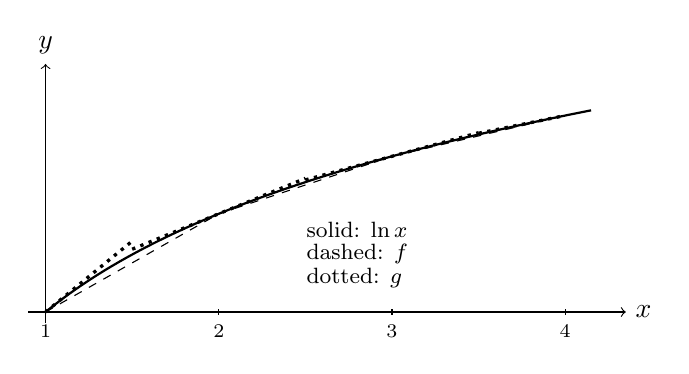
\begin{tikzpicture}[x=2.2cm,y=1.8cm,baseline=(current bounding box.center)]
 \draw[->] (0.9, 0) -- (4.35, 0) node[right] {$x$};
 \draw[->] (1, -0.08) -- (1, 1.75) node[above] {$y$};
 \foreach \m in {1, 2, 3, 4} {\draw (\m, 0.02)--(\m, -0.02) node[below] {\scriptsize $\m$};}
 \draw[thick] plot[domain=1:4.15, samples=75] (\x, {ln(\x)});
 \draw[dashed] (1, 0)--(2, {ln(2)})--(3, {ln(3)})--(4, {ln(4)});
 \draw[dotted, very thick] (1, 0)--(1.5, 0.5);
 \draw[dotted, very thick] (1.5, {1.5/2-1+ln(2)})--(2.5, {2.5/2-1+ln(2)});
 \draw[dotted, very thick] (2.5, {2.5/3-1+ln(3)})--(3.5, {3.5/3-1+ln(3)});
 \draw[dotted, very thick] (3.5, {3.5/4-1+ln(4)})--(4, {ln(4)});
 \node[anchor=west] at (2.45, 0.58) {\footnotesize solid: $\ln x$};
 \node[anchor=west] at (2.45, 0.41) {\footnotesize dashed: $f$};
 \node[anchor=west] at (2.45, 0.24) {\footnotesize dotted: $g$};
\end{tikzpicture}
\]
Since $\ln$ is strictly concave, each chord lies below its graph and each tangent lies above it. Thus $f\le\ln x\le g$, with strict inequalities except at certain integers.

On $[m, m+1]$ the integral of the linear interpolant is the average of its endpoint values:
\[
 \int_m^{m+1}f(x)\,\dd x=\frac{\ln m+\ln(m+1)}2.
\]
Summing from $m=1$ to $n-1$ gives $\int_1^nf=\ln(n!)-\frac12\ln n$. For $g$, the tangent at $m$ integrates to $\ln m$ on the full interval $[m-1/2, m+1/2]$. The half intervals at $1$ and $n$ give
\[
 \int_1^ng(x)\,\dd x=\ln(n!)-\frac12\ln n+\frac18\left(1-\frac1n\right).
\]
In particular $\int_1^nf>\int_1^ng-1/8$, as stated. Now integrate $\ln x$:
\[
 \ln(n!)-\frac12\ln n
 <\int_1^n\ln x\,\dd x=n\ln n-n+1
 <\int_1^ng(x)\,\dd x.
\]
Writing $A_n=\ln(n!)-(n+\tfrac12)\ln n+n$, the left inequality gives $A_n<1$; the right yields
\[
 A_n>1-\frac18\left(1-\frac1n\right)>\frac78.
\]
Exponentiating the resulting strict bounds gives the displayed approximation to Stirling's formula.
\end{solution}

\begin{exercise}{8.21}
Let
\[
 L_n=\frac1{2\pi}\int_{-\pi}^\pi|D_n(t)|\,\dd t\qquad(n=1, 2, 3, \ldots).
\]
Prove that there exists a constant $C>0$ such that $L_n>C\ln n$ for $n=1, 2, 3, \ldots$, or, more precisely, that the sequence
\[
 \left\{L_n-\frac4{\pi^2}\ln n\right\}
\]
is bounded.
\end{exercise}
\begin{solution}
Recall from (77) that $D_n(t)=\sin((n+\frac12)t)/\sin(t/2)$. By evenness, with $m=n+\frac12$,
\[
 L_n=\frac1\pi\int_0^\pi\frac{|\sin(mt)|}{\sin(t/2)}\,\dd t.
\]
On $(0, \pi]$ we can write
\[
 \frac1{\sin(t/2)}=\frac2t+r(t),
\]
where $r$ is bounded: near $0$, $\sin(t/2)=t/2+O(t^3)$, so $r(t)=O(t)$; away from $0$ the difference is continuous. Because $|\sin(mt)|\le1$,
\[
 L_n=\frac2\pi\int_0^\pi\frac{|\sin(mt)|}{t}\,\dd t+O(1)
 =\frac2\pi\int_0^{m\pi}\frac{|\sin u|}{u}\,\dd u+O(1),
\]
with error bounded independently of $n$.

The function $|\sin u|$ has period $\pi$ and mean $2/\pi$. Put $h(u)=|\sin u|-2/\pi$. Its integral over every full period is zero, so $H(v)=\int_0^v h(u)\,\dd u$ is bounded. Integration by parts, for $M\ge1$, yields
\[
 \int_1^M\frac{h(u)}u\,\dd u
 =\frac{H(M)}M-H(1)+\int_1^M\frac{H(u)}{u^2}\,\dd u=O(1).
\]
Since $\int_0^1|\sin u|/u\,\dd u$ is finite, we conclude
\[
 \int_0^M\frac{|\sin u|}u\,\dd u
 =\frac2\pi\ln M+O(1).
\]
Taking $M=m\pi$ and using $\ln(m\pi)=\ln n+O(1)$ gives
\[
 L_n=\frac4{\pi^2}\ln n+O(1).
\]
This proves the more precise boundedness assertion. In particular the ratio $L_n/\ln n$ tends to $4/\pi^2>0$ (for $n\ge2$), so a sufficiently small $C>0$ gives $L_n>C\ln n$ for all $n\ge2$; for $n=1$ the right side is zero and $L_1>0$.
\end{solution}

\begin{exercise}{8.22}
If $\alpha$ is real and $-1<x<1$, prove Newton's binomial theorem
\[
 (1+x)^\alpha=1+\sum_{n=1}^\infty
 \frac{\alpha(\alpha-1)\cdots(\alpha-n+1)}{n!}\,x^n.
\]
Show also that
\[
 (1-x)^{-\alpha}=\sum_{n=0}^\infty\frac{\Gamma(n+\alpha)}{n!\,\Gamma(\alpha)}x^n
\]
if $-1<x<1$ and $\alpha>0$.
\end{exercise}
\begin{solution}
Let $a_0=1$ and $a_n=\alpha(\alpha-1)\cdots(\alpha-n+1)/n!$ for $n\ge1$. The recurrence
\[
 (n+1)a_{n+1}=(\alpha-n)a_n
\]
shows that $|a_{n+1}/a_n|=|\alpha-n|/(n+1)\to1$ whenever the coefficients do not eventually vanish. Thus the ratio test establishes absolute convergence for $|x|<1$; if $\alpha$ is a nonnegative integer, the series is a polynomial instead. The differentiated power series has the same radius of convergence.

Writing $f(x)=\sum_{n\ge0}a_nx^n$ and comparing the coefficient of $x^n$ in $(1+x)f'(x)$ gives
\[
 (n+1)a_{n+1}+na_n=\alpha a_n.
\]
Hence $(1+x)f'(x)=\alpha f(x)$ on $(-1, 1)$. Multiplying the equation by $(1+x)^{-\alpha-1}$,
\[
 \frac{\dd}{\dd x}\bigl((1+x)^{-\alpha}f(x)\bigr)=0.
\]
Since $f(0)=1$, the constant is $1$; thus $f(x)=(1+x)^\alpha$.

For the second identity, replace $\alpha$ by $-\alpha$ and $x$ by $-x$. The coefficient becomes
\[
 (-1)^n\frac{(-\alpha)(-\alpha-1)\cdots(-\alpha-n+1)}{n!}
 =\frac{\alpha(\alpha+1)\cdots(\alpha+n-1)}{n!}
 =\frac{\Gamma(n+\alpha)}{n!\,\Gamma(\alpha)},
\]
using $\Gamma(u+1)=u\Gamma(u)$, valid here since $\alpha>0$. This establishes the Gamma-series formula.
\end{solution}

\begin{exercise}{8.23}
Let $\gamma$ be a continuously differentiable closed curve in the complex plane, with parameter interval $[a, b]$, and assume that $\gamma(t)\ne0$ for every $t\in[a, b]$. Define the index of $\gamma$ about the origin by
\[
 \Ind(\gamma, 0)=\frac1{2\pi i}\int_a^b\frac{\gamma'(t)}{\gamma(t)}\,\dd t.
\]
Prove that $\Ind(\gamma, 0)$ is always an integer.

Compute $\Ind(\gamma, 0)$ when $\gamma(t)=e^{int}$, $n\in\Z$, $a=0$, and $b=2\pi$.

Explain why this index is called the winding number about the origin.
\end{exercise}
\begin{solution}
Define
\[
 \varphi(t)=\int_a^t\frac{\gamma'(s)}{\gamma(s)}\,\dd s.
\]
The integrand is continuous since $\gamma$ is continuously differentiable and never vanishes, so $\varphi'=\gamma'/\gamma$ and $\varphi(a)=0$. By the product rule,
\[
 \frac{\dd}{\dd t}\bigl(\gamma(t)e^{-\varphi(t)}\bigr)
 =e^{-\varphi(t)}\bigl(\gamma'(t)-\gamma(t)\varphi'(t)\bigr)=0.
\]
Thus $\gamma(t)e^{-\varphi(t)}=\gamma(a)$. At $t=b$, because $\gamma(b)=\gamma(a)\ne0$, we have $e^{\varphi(b)}=1$. The complex exponential takes the value $1$ precisely at integer multiples of $2\pi i$. Therefore
\[
 \varphi(b)=2\pi i k\quad(k\in\Z), \qquad
 \Ind(\gamma, 0)=\frac{\varphi(b)}{2\pi i}=k\in\Z.
\]
For $\gamma(t)=e^{int}$ on $[0, 2\pi]$, $\gamma'/\gamma=in$, and hence
\[
 \Ind(\gamma, 0)=\frac1{2\pi i}\int_0^{2\pi}in\,\dd t=n
\]
(for integer $n$, so the curve is closed). This curve runs around the origin $n$ times, counterclockwise when $n>0$ and clockwise when $n<0$.
\end{solution}

\begin{exercise}{8.24}
Let $\gamma$ be as in Exercise 23, and assume in addition that the range of $\gamma$ does not intersect the negative real axis. Prove that $\Ind(\gamma, 0)=0$.
\end{exercise}
\begin{solution}
For every $c\ge0$, the curve $\gamma+c$ is closed, continuously differentiable, and nonvanishing: if $\gamma(t)+c=0$, then $\gamma(t)=-c$ lies on the forbidden negative real axis (including $0$). Thus Exercise 8.23 shows that
\[
 I(c):=\Ind(\gamma+c, 0)
 =\frac1{2\pi i}\int_a^b\frac{\gamma'(t)}{\gamma(t)+c}\,\dd t
\]
is an integer. The integrand depends continuously on $c$, uniformly in $t$ over compact parameter ranges; hence $I$ is continuous on $[0, \infty)$. A continuous integer-valued function on an interval is constant.

Let $M=\max_{t\in[a, b]}|\gamma(t)|$. For $c>M$,
\[
 |I(c)|\le\frac1{2\pi}\int_a^b\frac{|\gamma'(t)|}{c-M}\,\dd t
 \longrightarrow0\qquad(c\to\infty).
\]
Since $I(c)$ is constant and integer-valued, its constant value is $0$. In particular, $\Ind(\gamma, 0)=I(0)=0$.
\end{solution}

\begin{exercise}{8.25}
Suppose $\gamma_1$ and $\gamma_2$ are curves as in Exercise 23, and
\[
 |\gamma_1(t)-\gamma_2(t)|<|\gamma_1(t)|\qquad(a\le t\le b).
\]
Prove that $\Ind(\gamma_1, 0)=\Ind(\gamma_2, 0)$.
\end{exercise}
\begin{solution}
The ratio $\gamma=\gamma_2/\gamma_1$ is a continuously differentiable closed curve. It is well-defined because $\gamma_1$ never vanishes. Moreover,
\[
 |\gamma(t)-1|=\frac{|\gamma_2(t)-\gamma_1(t)|}{|\gamma_1(t)|}<1.
\]
Thus its range lies in the open disk $|z-1|<1$, contained entirely in the right half-plane, and so avoids the negative real axis. By Exercise 8.24, $\Ind(\gamma, 0)=0$.

The quotient rule gives
\[
 \frac{\gamma'}\gamma=\frac{\gamma_2'}{\gamma_2}-\frac{\gamma_1'}{\gamma_1}.
\]
Integrating over $[a, b]$ and dividing by $2\pi i$ yields
\[
 0=\Ind(\gamma, 0)
 =\Ind(\gamma_2, 0)-\Ind(\gamma_1, 0),
\]
which is the desired equality.
\end{solution}

\begin{exercise}{8.26}
Let $\gamma$ be a closed curve in the complex plane (not necessarily differentiable) with parameter interval $[0, 2\pi]$, such that $\gamma(t)\ne0$ for every $t\in[0, 2\pi]$.

Choose $\delta>0$ so that $|\gamma(t)|>\delta$ for all $t\in[0, 2\pi]$. If $P_1$ and $P_2$ are trigonometric polynomials such that $|P_j(t)-\gamma(t)|<\delta/4$ for all $t\in[0, 2\pi]$ ($j=1, 2$; their existence is assured by Theorem 8.15), prove that
\[
 \Ind(P_1, 0)=\Ind(P_2, 0)
\]
by applying Exercise 25.

Define this common value to be $\Ind(\gamma, 0)$.

Prove that the statements of Exercises 24 and 25 hold without any differentiability assumption.
\end{exercise}
\begin{solution}
The continuous nonvanishing curve $\gamma$ has $m=\min_t|\gamma(t)|>0$, so the stipulated $\delta$ exists. The trigonometric polynomials $P_j$ are continuously differentiable and periodic, and satisfy
\[
 |P_1(t)|\ge|\gamma(t)|-|P_1(t)-\gamma(t)|>\frac{3\delta}4,
 \qquad |P_2(t)-P_1(t)|<\frac\delta2<|P_1(t)|.
\]
Exercise 8.25 therefore gives $\Ind(P_1, 0)=\Ind(P_2, 0)$. This proves that defining $\Ind(\gamma, 0)$ by a sufficiently close trigonometric polynomial is independent of the choice of approximant. If $\gamma$ itself is continuously differentiable, a close approximant has the same index as $\gamma$ by Exercise 8.25, so the definition extends the old one.

We use the following direct consequence of the definition: if $\eta_1, \eta_2$ are continuous nonvanishing closed curves and
$|\eta_1(t)-\eta_2(t)|<|\eta_1(t)|$ at every $t$, then
$\Ind(\eta_1, 0)=\Ind(\eta_2, 0)$. Indeed, compactness makes the inequality uniformly strict. Approximate both curves sufficiently closely by trigonometric polynomials so that the strict inequality persists, apply Exercise 8.25 to the approximants, and then use the definition of their indices. This proves the continuous-curve version of Exercise 8.25.

For Exercise 8.24, suppose $\gamma$ is continuous and its range avoids the negative real axis. For every $c\ge0$, $\gamma+c$ is nonvanishing. Its index is locally constant in $c$, by the preceding stability statement and uniform continuity in $c$. Since $[0, \infty)$ is connected, the index is constant in $c$. For sufficiently large $c$, the curve $\gamma+c$ lies in the right half-plane; its trigonometric approximant may also be chosen there, and Exercise 8.24 for differentiable curves makes its index $0$. Thus $\Ind(\gamma, 0)=0$, as required.
\end{solution}

\begin{exercise}{8.27}
Let $f$ be a continuous complex function defined in the complex plane. Suppose there is a positive integer $n$ and a complex number $c\ne0$ such that
\[
 \lim_{|z|\to\infty}z^{-n}f(z)=c.
\]
Prove that $f(z)=0$ for at least one complex number $z$.

\end{exercise}
\begin{solution}
Assume, toward a contradiction, that $f$ has no zero. For $r\ge0$, define $\gamma_r(t)=f(re^{it})$ on $[0, 2\pi]$. Each $\gamma_r$ is then a continuous nonvanishing closed curve, so its index is defined by Exercise 8.26.

For $r=0$, $\gamma_0(t)=f(0)$ is constant and nonzero, so $\Ind(\gamma_0, 0)=0$.

The hypothesis at infinity implies, uniformly for $t\in[0, 2\pi]$,
\[
 \frac{f(re^{it})}{r^ne^{int}}\longrightarrow c.
\]
Thus, for all sufficiently large $r$,
\[
 |\gamma_r(t)-cr^ne^{int}|<|c|r^n
 \qquad(0\le t\le2\pi).
\]
By the continuous-curve stability result of Exercise 8.26, $\Ind(\gamma_r, 0)$ equals the index of $cr^ne^{int}$ about $0$, namely $n$ by Exercise 8.23.

Fix $r_0\ge0$. On a compact annulus around $r_0$ (a disk if $r_0=0$), $f$ is uniformly continuous, while $m_0=\min_t|\gamma_{r_0}(t)|>0$. Hence for $r$ sufficiently near $r_0$,
\[
 \sup_t|\gamma_r(t)-\gamma_{r_0}(t)|<m_0.
\]
Exercise 8.26 then gives $\Ind(\gamma_r, 0)=\Ind(\gamma_{r_0}, 0)$. Thus the integer-valued index is locally constant, in particular continuous, as a function of $r$.

Since $[0, \infty)$ is connected, a continuous integer-valued function on it must be constant. But the index equals $0$ at $r=0$ and equals $n>0$ for all sufficiently large $r$, a contradiction. Therefore $f$ vanishes somewhere.
\end{solution}

\begin{exercise}{8.28}
Let $D$ be the closed unit disc in the complex plane. (Thus $z\in D$ if and only if $|z|\le1$.) Let $g$ be a continuous mapping of $D$ into the unit circle $T$. (Thus $|g(z)|=1$ for every $z\in D$.)

Prove that $g(z)=-z$ for at least one $z\in T$.
\end{exercise}
\begin{solution}
Suppose that $g(z)\ne-z$ for all $z\in T$. The curves $\gamma_r(t)=g(re^{it})$ are continuous, closed, and nonvanishing (indeed, $|\gamma_r|=1$). The same argument as in Exercise 8.27(c), using Exercise 8.26, shows that $r\mapsto\Ind(\gamma_r, 0)$ is continuous and integer-valued. Hence it is constant on $[0, 1]$. Since $\gamma_0$ is the constant curve $g(0)$, we obtain
\[
 \Ind(\gamma_1, 0)=\Ind(\gamma_0, 0)=0.
\]
On the other hand, put $\varphi(t)=e^{-it}\gamma_1(t)$. This is a continuous closed curve with $|\varphi(t)|=1$, and $\varphi(t)\ne-1$ by assumption. As the only point of the negative real axis on the unit circle is $-1$, Exercises 8.24 and 8.26 imply $\Ind(\varphi, 0)=0$.

Indices of products add also for continuous nonvanishing curves: approximate each factor uniformly by a nonvanishing trigonometric polynomial. The product of the approximants is again a nonvanishing trigonometric polynomial, close to the product curve, and for these differentiable approximants the logarithmic derivative gives $\Ind(pq, 0)=\Ind(p, 0)+\Ind(q, 0)$. Passing to indices by Exercise 8.26 proves the rule. Since $\gamma_1(t)=e^{it}\varphi(t)$, Exercise 8.23 gives
\[
 \Ind(\gamma_1, 0)=\Ind(e^{it}, 0)+\Ind(\varphi, 0)=1+0=1.
\]
This contradicts the preceding value $0$. Consequently $g(z)=-z$ for some point $z$ of the unit circle.
\end{solution}

\begin{exercise}{8.29}
Let $D=\{z\in\C:|z|\le1\}$. Prove that every continuous mapping $f\colon D\to D$ has a fixed point.
\end{exercise}
\begin{solution}
Suppose $f(z)\ne z$ for every $z\in D$. Fix $z\in D$ and put $d(z)=z-f(z)\ne0$. Starting at $f(z)$ and moving through $z$ along the ray eventually reaches the unit circle at a unique point
\[
 g(z)=z+s(z)d(z), \qquad s(z)\ge0.
\]
Indeed, the equation $|z+sd|=1$ becomes
\[
 |d|^2s^2+2\RePart(z\overline d)s+|z|^2-1=0.
\]
For $|z|<1$, the constant term is negative, so there is precisely one positive root. At $|z|=1$, the point $z$ already lies on the circle, and $s=0$ is the desired root. In this boundary case
\[
 \RePart(z\overline d)=1-\RePart(z\overline{f(z)})>0,
\]
since $|f(z)|\le1$ and $f(z)\ne z$. Thus the nonnegative root is uniquely given everywhere by
\[
 s(z)=\frac{-\RePart(z\overline{d(z)})
 +\sqrt{\RePart(z\overline{d(z)})^2+|d(z)|^2(1-|z|^2)}}{|d(z)|^2}.
\]
The denominator never vanishes, so this formula shows that $s$ and $g$ are continuous on $D$. By construction $|g(z)|=1$; also $g(z)=z$ for $z\in T$. Hence $g\colon D\to T$ is a continuous map restricting to the identity on $T$.

Exercise 8.28 applied to $g$ asserts that $g(z)=-z$ for some $z\in T$. But there $g(z)=z$, so $z=-z$, impossible when $|z|=1$. The assumption was false, and $f$ has a fixed point.
\end{solution}

\begin{exercise}{8.30}
Use Stirling's formula to prove that
\[
 \lim_{x\to\infty}\frac{\Gamma(x+c)}{x^c\Gamma(x)}=1
\]
for every real constant $c$.
\end{exercise}
\begin{solution}
For sufficiently large $x$, both $x$ and $x+c$ are positive. Stirling's formula gives
\[
 \Gamma(u)\sim\sqrt{2\pi}\,u^{u-1/2}e^{-u}\qquad(u\to\infty).
\]
Applying it at $u=x+c$ and $u=x$ and cancelling common factors yields
\[
 \frac{\Gamma(x+c)}{x^c\Gamma(x)}
 \sim e^{-c}\left(1+\frac cx\right)^{x+c-1/2}.
\]
The logarithm of the expression on the right is
\[
 -c+\left(x+c-\frac12\right)\ln\left(1+\frac cx\right)
 =-c+\left(x+c-\frac12\right)\left(\frac cx+O(x^{-2})\right)\longrightarrow0.
\]
Exponentiating proves that the ratio tends to $1$, as required.
\end{solution}

\begin{exercise}{8.31}
In the proof of Theorem 7.26 it was shown that
\[
 \int_{-1}^1(1-x^2)^n\,\dd x\ge\frac4{3\sqrt n}
\]
for $n=1, 2, 3, \ldots$. Use Theorem 8.20 and Exercise 30 to show the more precise result
\[
 \lim_{n\to\infty}\sqrt n\int_{-1}^1(1-x^2)^n\,\dd x=\sqrt\pi.
\]
\end{exercise}
\begin{solution}
The integrand is even. Substitute $u=x^2$ on $[0, 1]$ to obtain
\[
 \begin{aligned}
 I_n:=\int_{-1}^1(1-x^2)^n\,\dd x
 &=2\int_0^1(1-x^2)^n\,\dd x\\
 &=\int_0^1u^{-1/2}(1-u)^n\,\dd u
 =B\left(\frac12, n+1\right).
 \end{aligned}
\]
The Beta--Gamma relation in Theorem 8.20 gives
\[
 I_n=\frac{\Gamma(1/2)\Gamma(n+1)}{\Gamma(n+3/2)}.
\]
Since $\Gamma(1/2)=\sqrt\pi$ and Exercise 8.30 with $x=n+1$, $c=1/2$ gives
\[
 \frac{\Gamma(n+3/2)}{(n+1)^{1/2}\Gamma(n+1)}\longrightarrow1,
\]
we conclude that
\[
 \sqrt n I_n
 =\sqrt\pi\,\sqrt{\frac n{n+1}}
 \frac{(n+1)^{1/2}\Gamma(n+1)}{\Gamma(n+3/2)}
 \longrightarrow\sqrt\pi.
\]
\end{solution}

\end{document}
